\documentclass{article}

\usepackage[preprint]{neurips_2026}

\usepackage[utf8]{inputenc}
\usepackage[T1]{fontenc}
\renewcommand{\ttdefault}{lmtt}
\usepackage{hyperref}
\usepackage{xurl}
\usepackage{booktabs}
\usepackage{amsfonts}
\usepackage{amsmath}
\usepackage{nicefrac}
\usepackage{microtype}
\usepackage{xcolor}
\usepackage{graphicx}
\usepackage{subcaption}

\graphicspath{{../figures/}}
\newcommand{\growE}{\textsc{Grow-early}}
\newcommand{\growL}{\textsc{Grow-late}}
\newcommand{\growVE}{\textsc{Grow-very-early}}
\newcommand{\growF}{\textsc{Grow-early-to-4}}
\newcommand{\growR}{\textsc{Grow-early-random}}
\newcommand{\coderepo}{\url{https://github.com/adlsdztony/depth-growth-vs-search}}

\hypersetup{colorlinks=true, linkcolor=blue!50!black, citecolor=blue!50!black, urlcolor=blue!50!black}

\usepackage{placeins}
\renewcommand{\topfraction}{0.9}
\renewcommand{\bottomfraction}{0.6}
\renewcommand{\textfraction}{0.1}
\renewcommand{\floatpagefraction}{0.85}
\setcounter{topnumber}{3}
\setcounter{totalnumber}{4}

\title{Grow Instead of Search? Function-Preserving\\Depth Growth for Multi-Task PPO on MT10}

\author{%
  Zicheng Gong\thanks{Equal contribution; authors are listed in alphabetical order of surname.} \qquad
  Zhewei Kang\footnotemark[1] \qquad
  Zilong Zhou\footnotemark[1]
}

\begin{document}

\maketitle

\begin{abstract}
The depth of a policy network is usually chosen by training one network per candidate depth and keeping the best one, which multiplies the cost of reinforcement-learning runs that are already expensive.
We ask whether a single run that starts shallow and grows deeper can replace this search when the cost of the search is counted.
New layers are inserted with an identity initialisation after a ReLU, which leaves the policy exactly unchanged and keeps the optimiser state of all existing weights.
On Meta-World MT10 with a multi-task PPO learner, we train actors of depth 1--4 and up to five growth variants at two widths for 3M environment steps each (80 runs in total), and evaluate on goal configurations held out from training and from model selection.
Depth is worth 24 points of held-out success (64\% at depth 1, 88\% at depth 4).
Growing from depth 1 to depth 4 early in training reaches 87.6\% in a single run, 1.4 points below the best fixed depth found by grid search, for 28\% of the learner compute of grid search and 56\% of the compute of successive halving.
The way layers are added matters: initialising the inserted layers randomly instead of as the identity costs 8.6 points, and inserting the same layers late costs 5.0 points.
With narrower actors (width 128), where depth 3 is best, the same schedule reaches 76.2\%, 4.8 points below grid search (not resolved with five seeds) at 26\% of its compute, so the advantage over a default depth is smaller there.
Code, per-run logs and scripts for every figure are available at \coderepo.
\end{abstract}

\section{Introduction}

The size of a deep reinforcement learning (RL) network is rarely tuned per problem, even though recent work shows that it matters a great deal when the network is designed to scale \citep{nauman2024bro,lee2025simba}.
The standard way to choose it is search: train one agent per candidate architecture and keep the one that does best on validation \citep{elsken2019nas}.
In RL each run consumes millions of simulator interactions and results are sensitive to the random seed \citep{henderson2018matters}, so a search over $K$ depths multiplies an already large cost by up to $K$.

Function-preserving growth \citep{chen2016net2net,wei2016morphism} suggests another route: start with a small network and add layers during training, initialised so that the function computed by the network does not change.
If a growing run reached the performance of the best depth, one run would replace $K$.
For RL this is not obvious.
A new layer starts with fresh optimiser statistics and has to become useful while the policy collects its own data, and networks trained with RL are known to lose plasticity as training proceeds \citep{nikishin2022primacy,lyle2023plasticity,dohare2024loss}.

We study this question in a controlled setting: a multi-task PPO learner \citep{schulman2017ppo,li2026toppo} on Meta-World MT10 \citep{yu2020metaworld}, where only the depth of the actor changes between runs.
Our framing is explicit about cost: \emph{the right depth is not known in advance, and the cost of a method includes all compute spent before a final policy is chosen}, including the runs a search throws away.
Under this framing a fixed depth is not a free baseline but a guess, and growth competes with search methods, not with the best depth in hindsight.

We set up a cost-aware protocol for choosing depth on MT10, with separate training, validation and held-out goals per task, and compare growth against grid search, successive halving and fixed guesses in environment steps and learner FLOPs (80 runs of 3M steps).
With width-400 actors, growing from depth 1 to depth 4 early in training comes within 1.4 points of the best fixed depth (not resolved with five seeds) at 28\% of the compute of grid search and 56\% of successive halving; with width-128 actors, where depth 3 is best, the same schedule stays 4.8 points below grid search (also not resolved).

How layers are added matters as much as whether they are added.
Initialising the new layers randomly instead of as the identity drops training success by 15--34 points at each insertion and costs 8.6 points at the end of training, and inserting the same layers late costs 5.0 points.

\begin{figure}[!t]
    \centering
    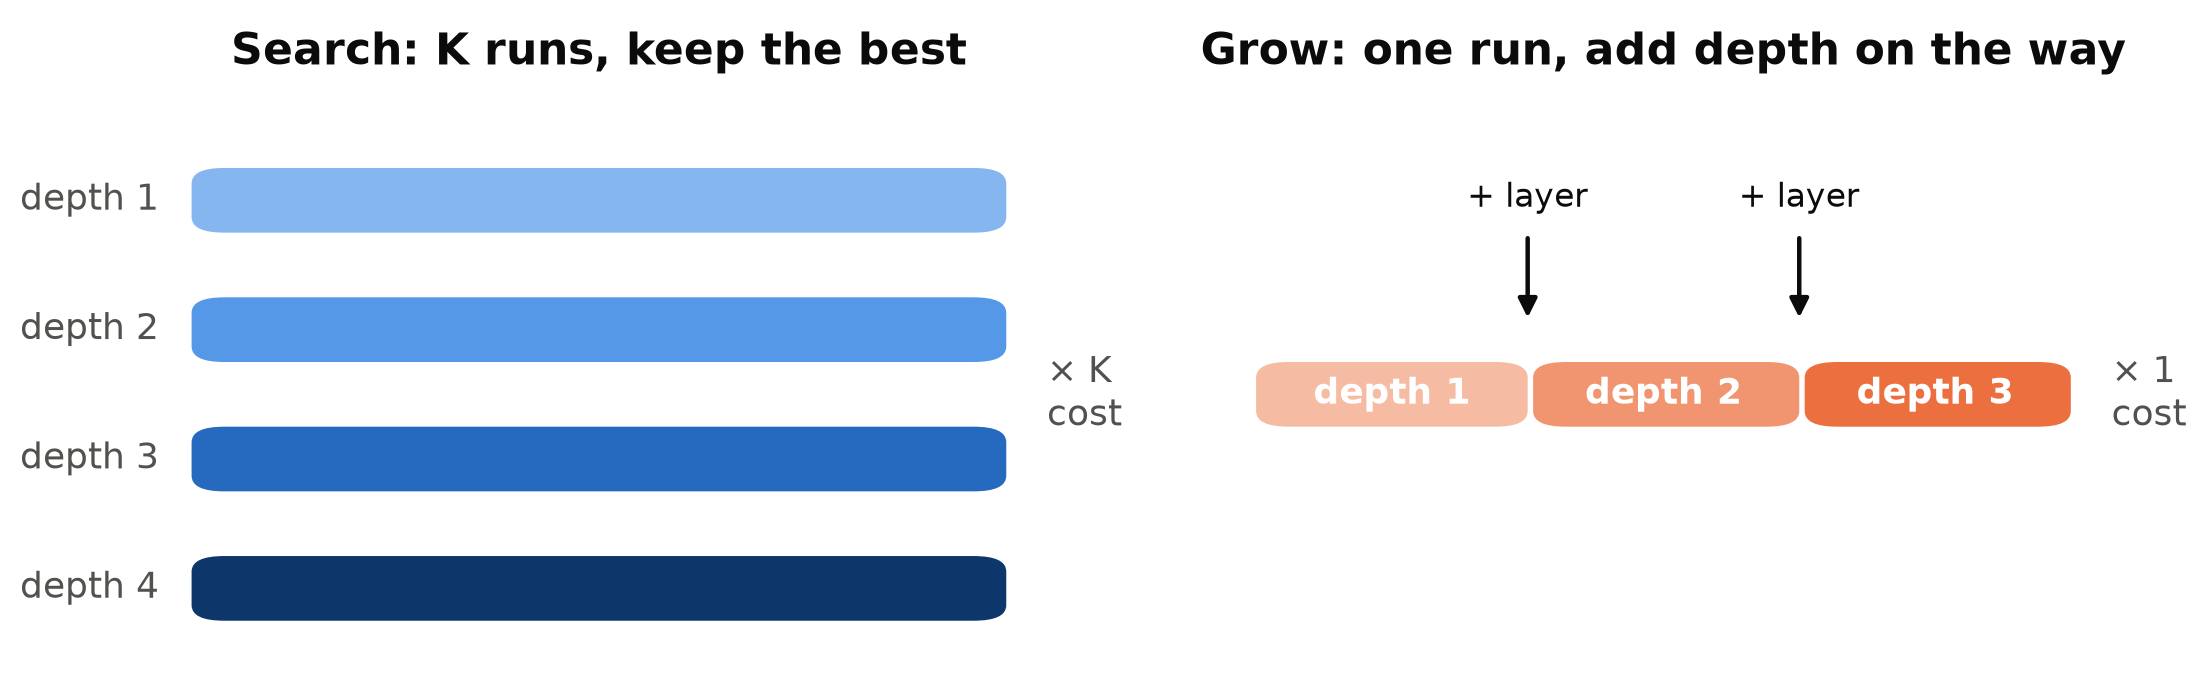
\includegraphics[width=0.85\linewidth]{static/schematic_search_vs_grow.png}\\[1mm]
    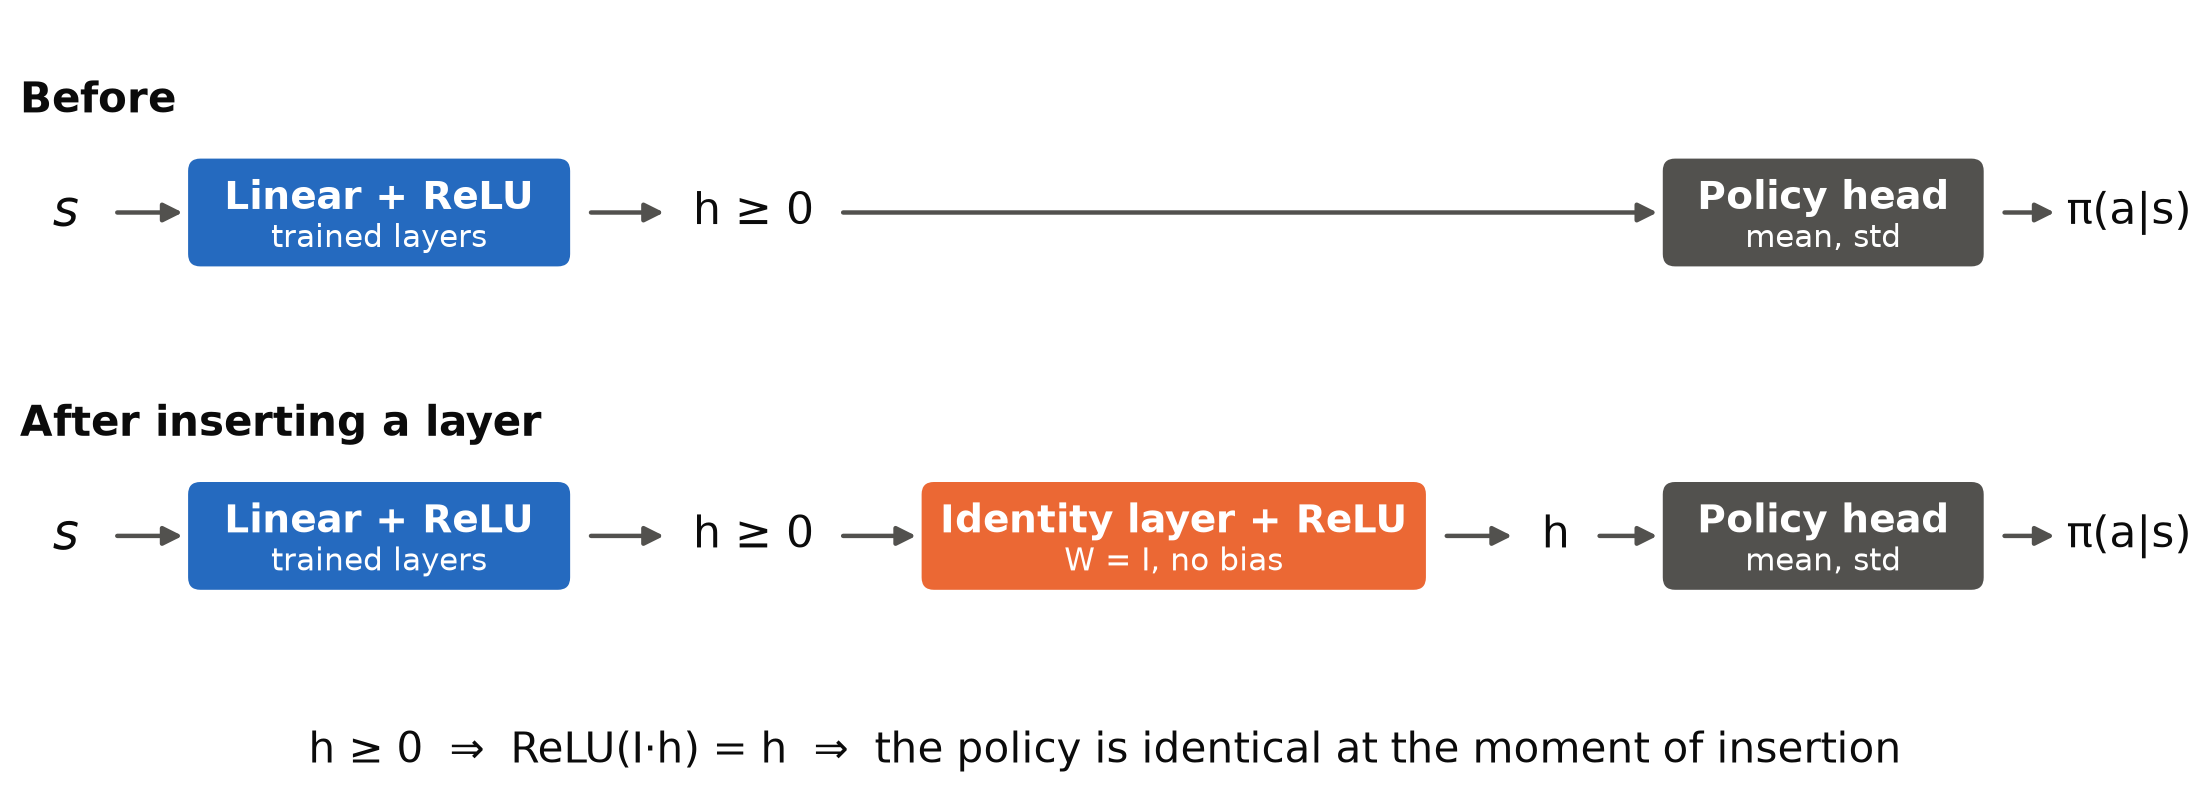
\includegraphics[width=0.8\linewidth]{static/identity_schematic.png}
    \caption{Top: a search trains one network per candidate depth; growth trains one network and adds layers on the way. Bottom: identity insertion. Because the hidden representation $h$ after a ReLU is non-negative, a new identity layer followed by a ReLU returns $h$ unchanged, so the policy is identical at the moment of insertion.}
    \label{fig:overview}
\end{figure}

\section{Related work}

\paragraph{Growing networks.}
Net2Net \citep{chen2016net2net} and network morphism \citep{wei2016morphism} introduced function-preserving widening and deepening, with identity initialisation for new layers.
Later methods choose where and how to grow from gradient information \citep{wu2020firefly,evci2022gradmax}, and progressive schemes grow generators \citep{karras2018progressive} or stack layers to cut the cost of training large language models \citep{gong2019stacking}.
These works mostly study supervised learning and ask whether growth reaches a \emph{chosen} larger network faster.
In RL, progressive networks \citep{rusu2016progressive} add a column per new task to avoid forgetting, which grows capacity across tasks rather than within one training run.
We ask a different question: whether growth can stand in for the \emph{choice} of the size, and we charge the alternative, search, for all its runs.

\paragraph{Hyperparameter search under a budget.}
Successive halving, Hyperband and their asynchronous variants \citep{jamieson2016sh,li2018hyperband,li2020asha} spend more budget on promising configurations and stop poor ones early; population-based training \citep{jaderberg2017pbt} adapts hyperparameters within a population of runs.
We use grid search and successive halving as baselines because they select among exactly the same fixed-depth runs and differ only in how much of each run they pay for.

\paragraph{Network scale and plasticity in RL.}
Larger networks help in continuous control when combined with normalisation and regularisation \citep{nauman2024bro,lee2025simba}, while RL training can reduce a network's ability to keep learning \citep{nikishin2022primacy,lyle2023plasticity,dohare2024loss}.
Our learner normalises per-task value targets with PopArt \citep{vanhasselt2016popart,hessel2019popart} and uses a LayerNorm critic \citep{ba2016layernorm}, following the reference implementation \citep{li2026toppo}.

\section{Method}

\paragraph{Problem.}
We are given $K$ candidate actor depths and a per-run budget of $T$ environment steps.
A strategy returns one policy; its quality is the success of that policy on held-out goals, and its cost is all environment steps and learner FLOPs it spent, including runs it discards.
Selection may use validation goals only.

\paragraph{Identity insertion.}
Let the actor body end with a hidden representation $h = \mathrm{ReLU}(z) \in \mathbb{R}_{\ge 0}^{W}$.
We append a bias-free linear layer $W_{\text{new}} \in \mathbb{R}^{W\times W}$ followed by a ReLU, initialised to $W_{\text{new}} = I$.
Because $h \ge 0$ element-wise,
\begin{equation}
    \mathrm{ReLU}(W_{\text{new}}\, h) = \mathrm{ReLU}(h) = h ,
\end{equation}
so the action mean, the state-independent action standard deviation and therefore the whole Gaussian policy are unchanged at insertion (Figure~\ref{fig:overview}).
The critic is not modified.
All existing parameters keep their Adam \citep{kingma2015adam} moment estimates; the new layer is added as a new parameter group with the same learning rate and fresh moments, and is included in gradient clipping.
Our implementation asserts at every insertion that the action mean changes by at most $10^{-5}$ on the current observations, that the action standard deviation and critic output are bit-identical, and that the optimiser state of existing parameters and the global random-number state are unchanged.
For the random-initialisation ablation we use PyTorch's default initialisation of a linear layer \citep{he2015delving} and keep everything else the same.

\paragraph{Growth schedules.}
All growth runs start at depth 1 and insert layers between PPO iterations, when the rollout buffer is empty.
\growE{} inserts at 0.5M and 1M steps (final depth 3); \growVE{} at 0.2M and 0.4M; \growL{} at 1M and 2M; \growF{} at 0.5M, 1M and 1.5M (final depth 4, the largest candidate depth).
\growR{} uses the schedule of \growE{} with randomly initialised layers.
The schedules are fixed in advance and do not look at validation success.

\section{Experimental setup}

\paragraph{Environment and learner.}
We use Meta-World MT10 \citep{yu2020metaworld} on MuJoCo \citep{todorov2012mujoco}: ten manipulation tasks learned by one policy that receives the 39-dimensional state and a one-hot task identifier and outputs a 4-dimensional action (Figure~\ref{fig:bench}).
The learner is the multi-task PPO of \citet{li2026toppo} with GAE \citep{schulman2016gae} ($\lambda = 0.97$, $\gamma = 0.99$), clip range 0.2, value clipping, entropy coefficient 0.005, learning rate $3\times10^{-4}$, 100k-step rollouts from 10 parallel environments (one per task), 16 epochs per rollout with stratified mini-batches of 3{,}125, PopArt value normalisation and a 3-layer, width-400 LayerNorm critic.
Only the actor's hidden depth (1--4 layers of width 400; a secondary study uses width 128) or its growth schedule differs between runs, and every run gets $T = 3$M environment steps.

\begin{figure}[!t]
    \centering
    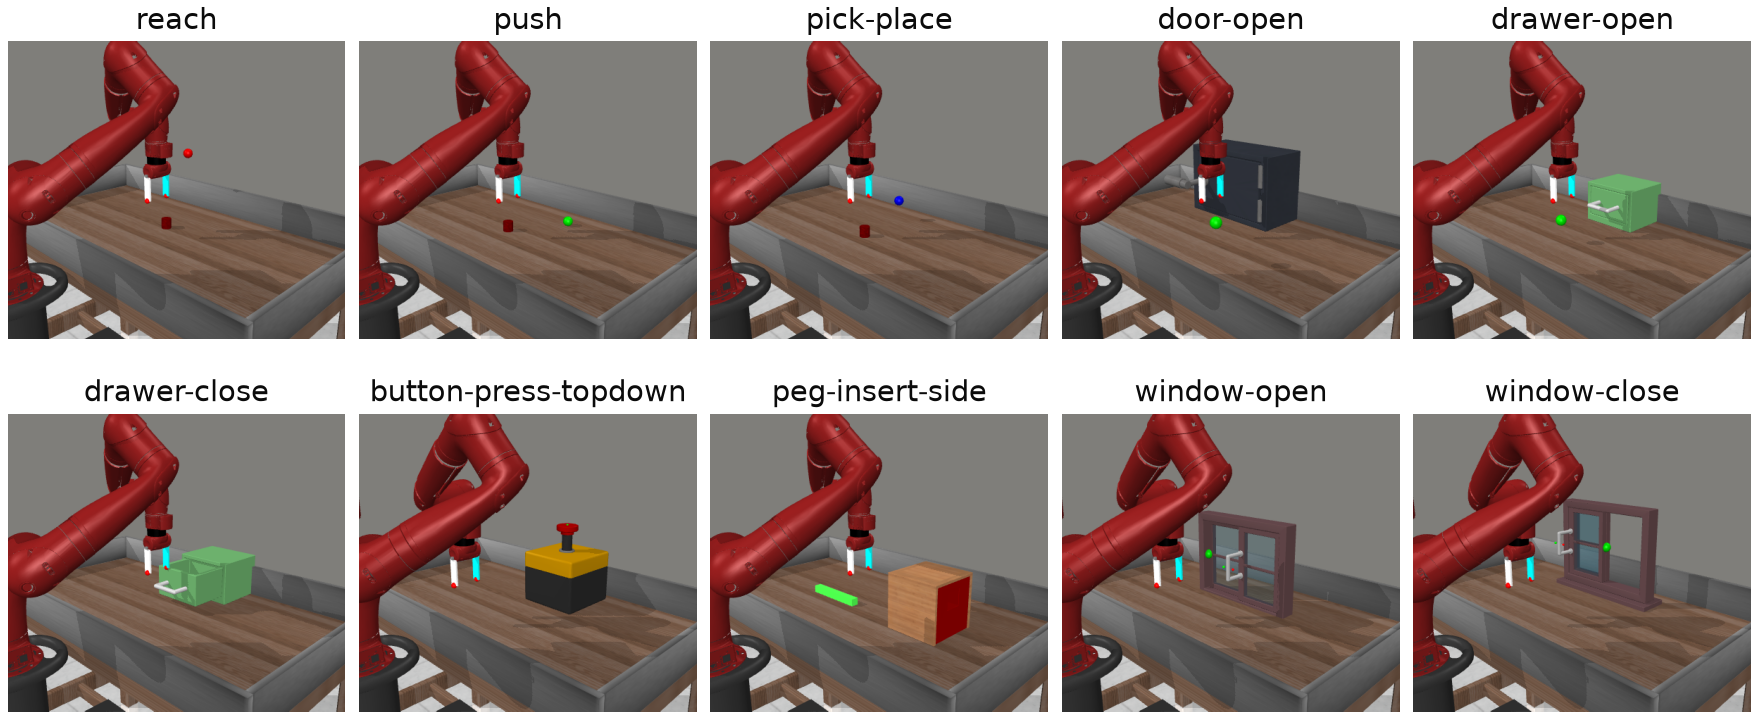
\includegraphics[width=\linewidth]{static/mt10_real.png}\\[1mm]
    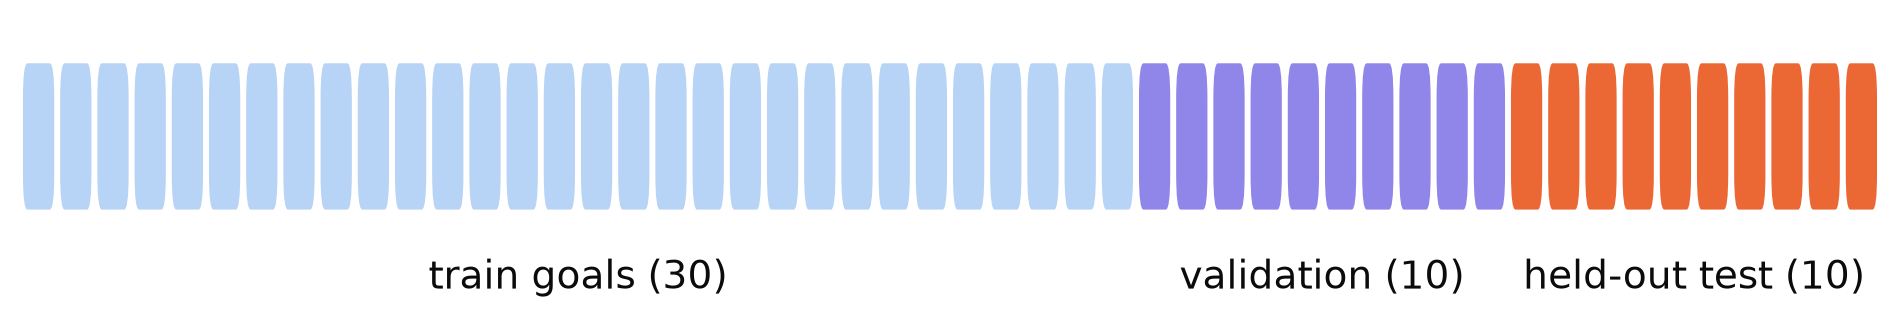
\includegraphics[width=0.65\linewidth]{static/goal_split.png}
    \caption{Top: the ten MT10 tasks, learned by a single policy. Bottom: per task, the 50 goal configurations (object and target positions) are split into 30 training, 10 validation and 10 held-out test goals.}
    \label{fig:bench}
\end{figure}

\paragraph{Goal split and evaluation.}
Each MT10 task has 50 goal configurations.
With a fixed benchmark seed we use goals 0--29 for training, 30--39 for validation and model selection, and 40--49 as held-out test goals.
Every 0.5M steps the evaluation-mode policy runs one episode on each of 10 training, 10 validation and 10 test goals of every task (300 episodes); success is Meta-World's binary success signal at any step of the 500-step episode.
All numbers are held-out test success unless stated otherwise.

\paragraph{Baselines.}
With $K=4$ candidate depths:
\emph{grid search} trains all four depths and returns the one with the best final validation success (cost $4T$);
\emph{successive halving} \citep{jamieson2016sh} trains all four depths to $T/6$, keeps the best two by validation success until $T/2$ and the best one until $T$ (cost $5.5$M steps).
It is simulated from the logged validation curves of the same runs, so it sees exactly the learning curves a real implementation with these rungs would see.
\emph{Default depth 2} is the depth of the reference recipe; \emph{random depth} is the mean over the four depths, the expected outcome of a guess.
\emph{Best fixed depth} picks the depth with the highest test success per seed; it is an upper reference, not an achievable method.
We use five seeds per configuration at both widths; all comparisons are paired by seed and we report 95\% $t$-intervals of paired differences \citep{agarwal2021precipice}.

\paragraph{Cost.}
We count environment steps and learner FLOPs.
Per training sample, the learner spends $2P$ FLOPs in the rollout forward pass and $16 \times 6P$ in the 16 PPO epochs, where $P$ is the number of actor plus critic parameters at that time, so a growing run pays for its small network while it is small.
FLOPs are independent of the hardware: our runs used RTX A6000, T4, RTX 4070 and RTX 3050 GPUs, and with a few hundred thousand parameters, measured GPU time was dominated by kernel-launch overhead and load on shared machines rather than by depth.
A 3M-step run took 35--65 minutes of wall-clock time, most of it CPU simulation.

\FloatBarrier
\section{Results}

\begin{figure}[!t]
    \centering
    \begin{subfigure}[t]{0.49\linewidth}
        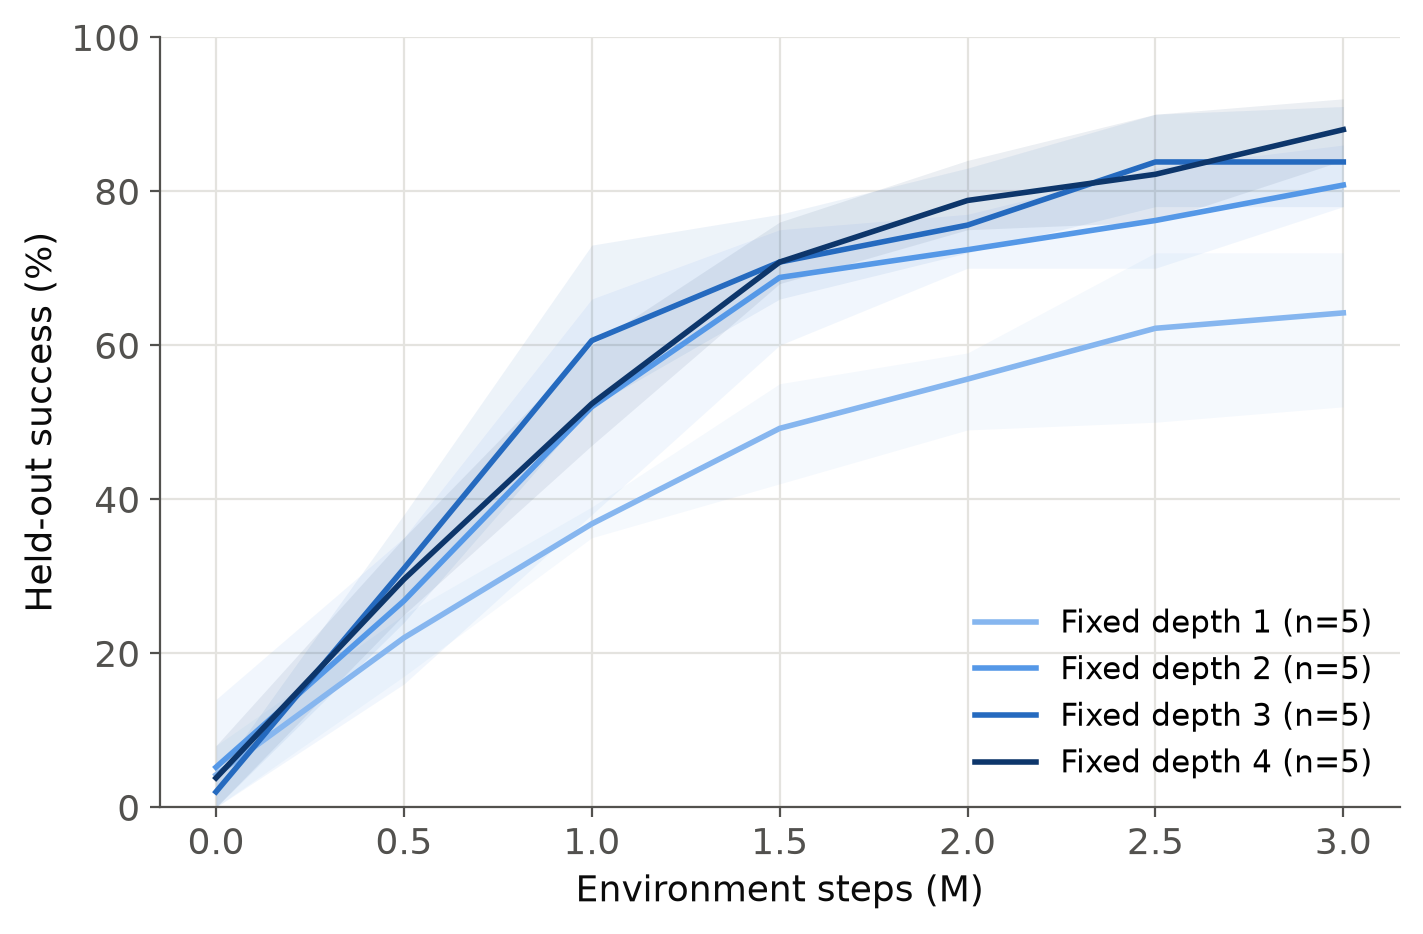
\includegraphics[width=\linewidth]{w400/curves_success_test.png}
        \caption{Held-out success during training}
        \label{fig:curves}
    \end{subfigure}\hfill
    \begin{subfigure}[t]{0.49\linewidth}
        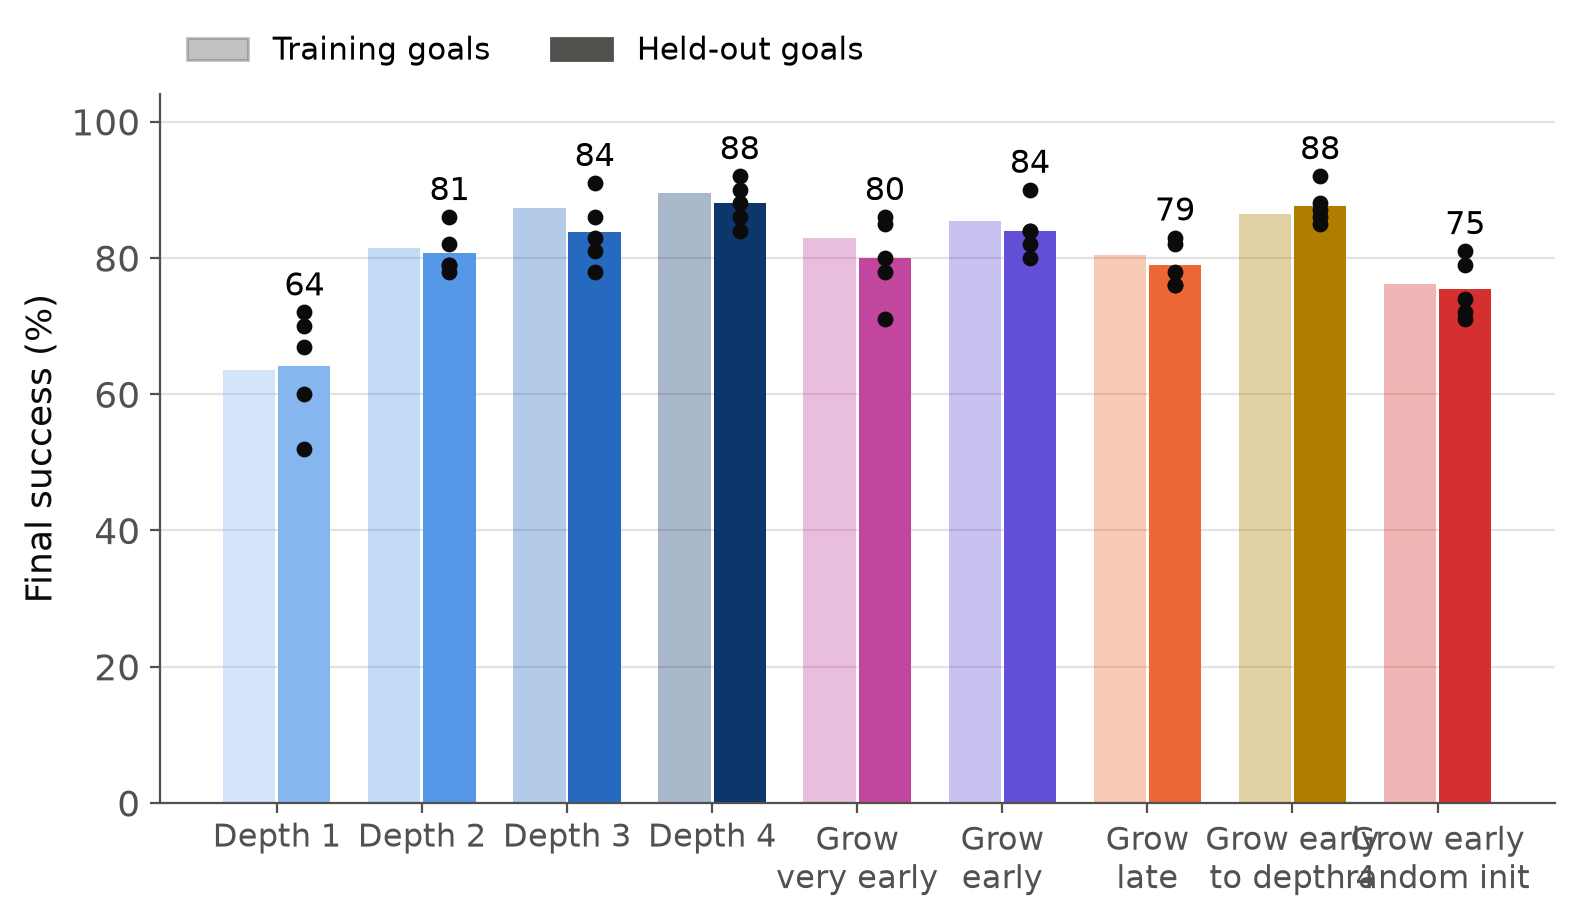
\includegraphics[width=\linewidth]{w400/final_train_vs_test.png}
        \caption{Final success, training vs.\ held-out goals}
        \label{fig:final}
    \end{subfigure}
    \caption{Width 400, five seeds. (a) Fixed depths, mean and range over seeds. (b) Light bars: training goals; dark bars: held-out goals; dots: individual seeds.}
    \label{fig:depth}
\end{figure}

\paragraph{Depth matters, and held-out goals are not harder than training goals.}
Final held-out success rises from 64\% at depth 1 to 81\%, 84\% and 88\% at depths 2--4 (Figure~\ref{fig:curves}).
The best depth in hindsight is 3 for two seeds and 4 for three, and validation selects the same depth as the test set in all five seeds.
Across all configurations, success on training goals and on held-out goals differs by at most 3.6 points (Figure~\ref{fig:final}): goal configurations within a task interpolate one another, so the split is a valid held-out test but does not make MT10 harder.
Per task (Figure~\ref{fig:pertask} in the appendix), six tasks are solved at every depth; the gains come from \texttt{peg-insert-side} (0\% $\to$ 76\%), \texttt{push} (22\% $\to$ 88\%) and \texttt{drawer-open} (40\% $\to$ 100\%), while \texttt{pick-place} stays at or below 18\% for every configuration within this budget.

\begin{figure}[!t]
    \centering
    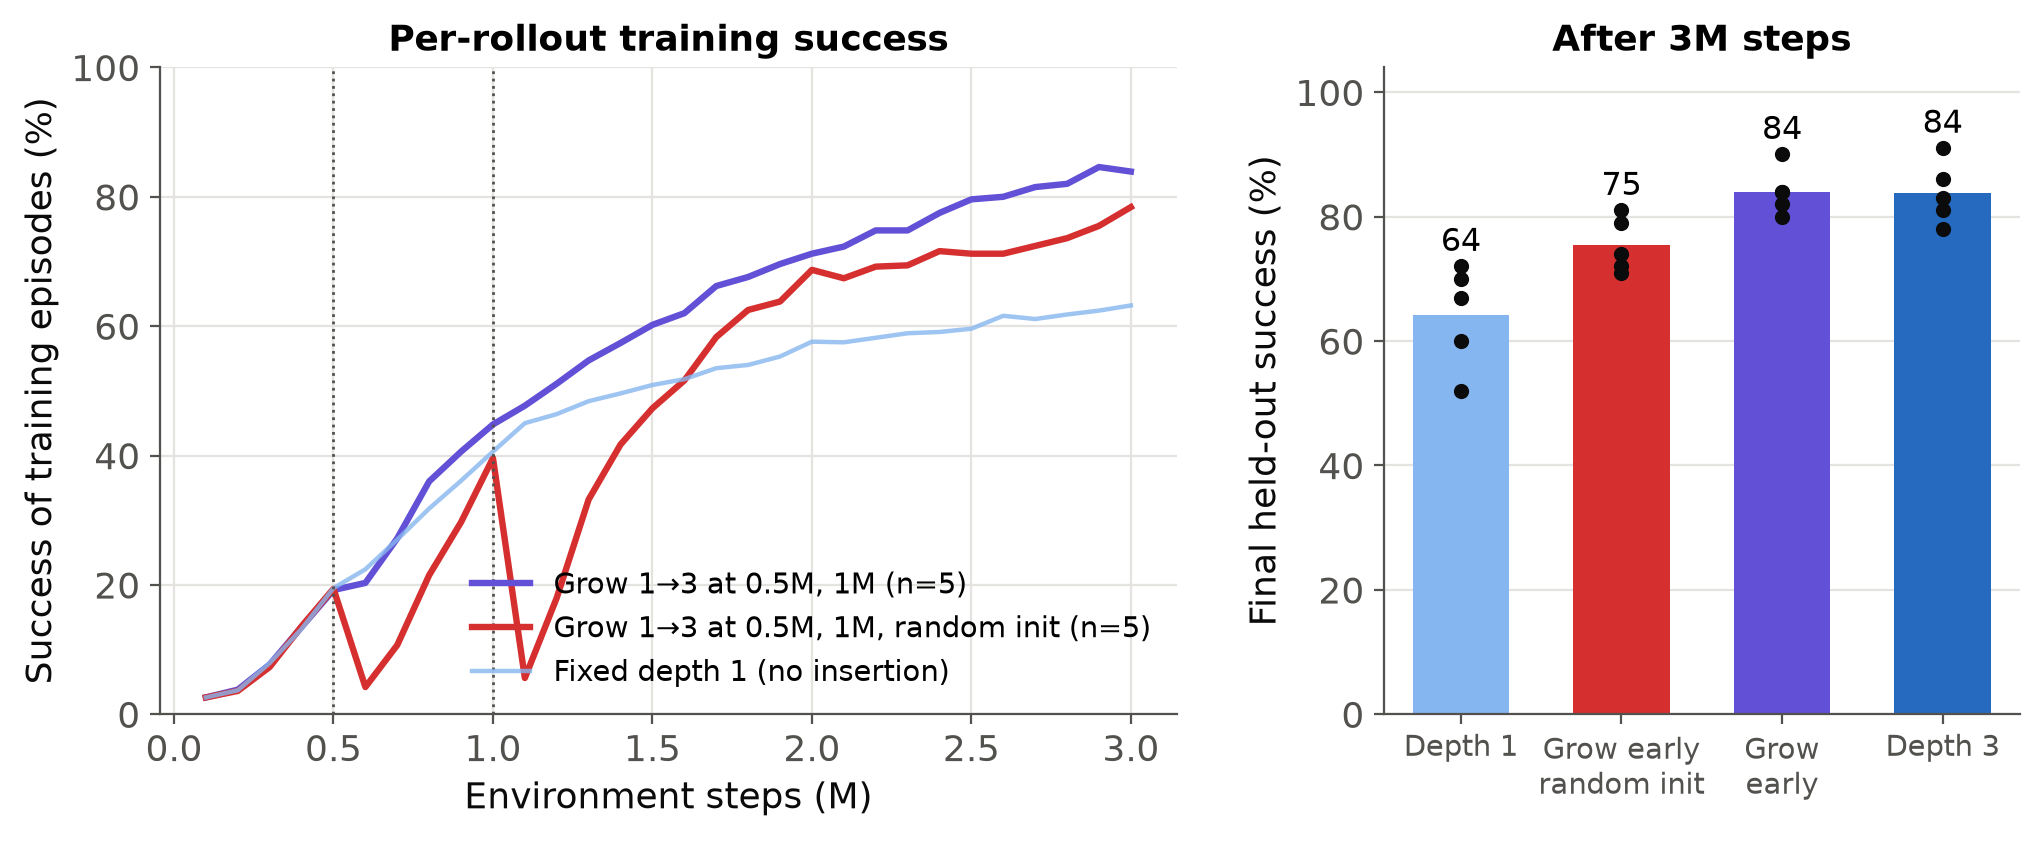
\includegraphics[width=\linewidth]{w400/insertion.png}
    \caption{Identity versus random initialisation of the inserted layers, both inserted at 0.5M and 1M steps (dotted lines), width 400, five seeds. Left: success of the training episodes completed in each 100k-step rollout, mean over seeds. Right: final held-out success; dots are seeds.}
    \label{fig:insertion}
\end{figure}

\paragraph{Identity initialisation is necessary.}
All 45 identity insertions at width 400 left the action mean unchanged to within floating-point precision (maximum error 0), and training success in the rollout after an insertion was on average $+1.1$ and $+2.9$ points above the rollout before it (first and second insertion).
Inserting randomly initialised layers at the same steps instead dropped training success by $15.2$ and $34.0$ points on average; after each insertion the runs took 0.4--0.5M steps to return to the level of fixed depth 1 and stayed below \growE{} for the rest of training (Figure~\ref{fig:insertion}).
At the end of training \growR{} reaches 75.4\%, $8.6 \pm 4.9$ points below \growE{}.
Its loss is concentrated on the hardest tasks: \texttt{peg-insert-side} 36\% versus 80\% and \texttt{push} 16\% versus 50\%.

\paragraph{When layers are added matters.}
Figure~\ref{fig:traj} in the appendix shows every growth run.
No run drops in held-out success after an identity insertion.
\growE{} reaches the level of fixed depth 3 (84.0\% vs.\ 83.8\%), while \growL{}, which spends only 1M steps at depth 3, ends at 79.0\%, the level of depth 2 and $5.0 \pm 3.0$ points below \growE{}.
Growing earlier than \growE{} did not help: \growVE{} reaches 80.0\%, with a large spread over seeds (71--86\%; difference to \growE{} $-4.0 \pm 10.8$).
Within the schedules we tried, inserting layers after 0.5M--1M steps works best, but our evidence does not identify a precise optimum.

\begin{table}[!t]
    \caption{Strategies for producing one policy without knowing the right depth (width 400, five paired seeds). Success is held-out test success at 3M steps of the returned policy (mean $\pm$ standard error). Costs include all runs a strategy trains. $^\dagger$Requires test results; not achievable without search. $^\ddagger$Ablation.}
    \label{tab:main}
    \centering
    \small
    \begin{tabular}{lccc}
        \toprule
        Strategy & Success (\%) & Env.\ steps (M) & Learner PFLOP \\
        \midrule
        Grid search, depths 1--4          & $89.0 \pm 1.3$ & 12.0 & 0.71 \\
        Successive halving (simulated)    & $85.2 \pm 2.9$ & 5.5  & 0.36 \\
        Default depth 2                   & $80.8 \pm 1.5$ & 3.0  & 0.15 \\
        Random depth (mean of 1--4)       & $79.2 \pm 1.1$ & 3.0  & 0.18 \\
        \midrule
        \growF{} (1$\to$4 at 0.5M, 1M, 1.5M) & $\mathbf{87.6 \pm 1.2}$ & 3.0 & 0.20 \\
        \growE{} (1$\to$3 at 0.5M, 1M)    & $84.0 \pm 1.7$ & 3.0  & 0.18 \\
        \growVE{} (1$\to$3 at 0.2M, 0.4M) & $80.0 \pm 2.7$ & 3.0  & 0.19 \\
        \growL{} (1$\to$3 at 1M, 2M)      & $79.0 \pm 1.5$ & 3.0  & 0.15 \\
        \growR{}$^\ddagger$ (random init)  & $75.4 \pm 2.0$ & 3.0  & 0.18 \\
        \midrule
        Best fixed depth$^\dagger$        & $89.0 \pm 1.3$ & 3.0  & 0.23 \\
        \bottomrule
    \end{tabular}
\end{table}

\begin{figure}[!t]
    \centering
    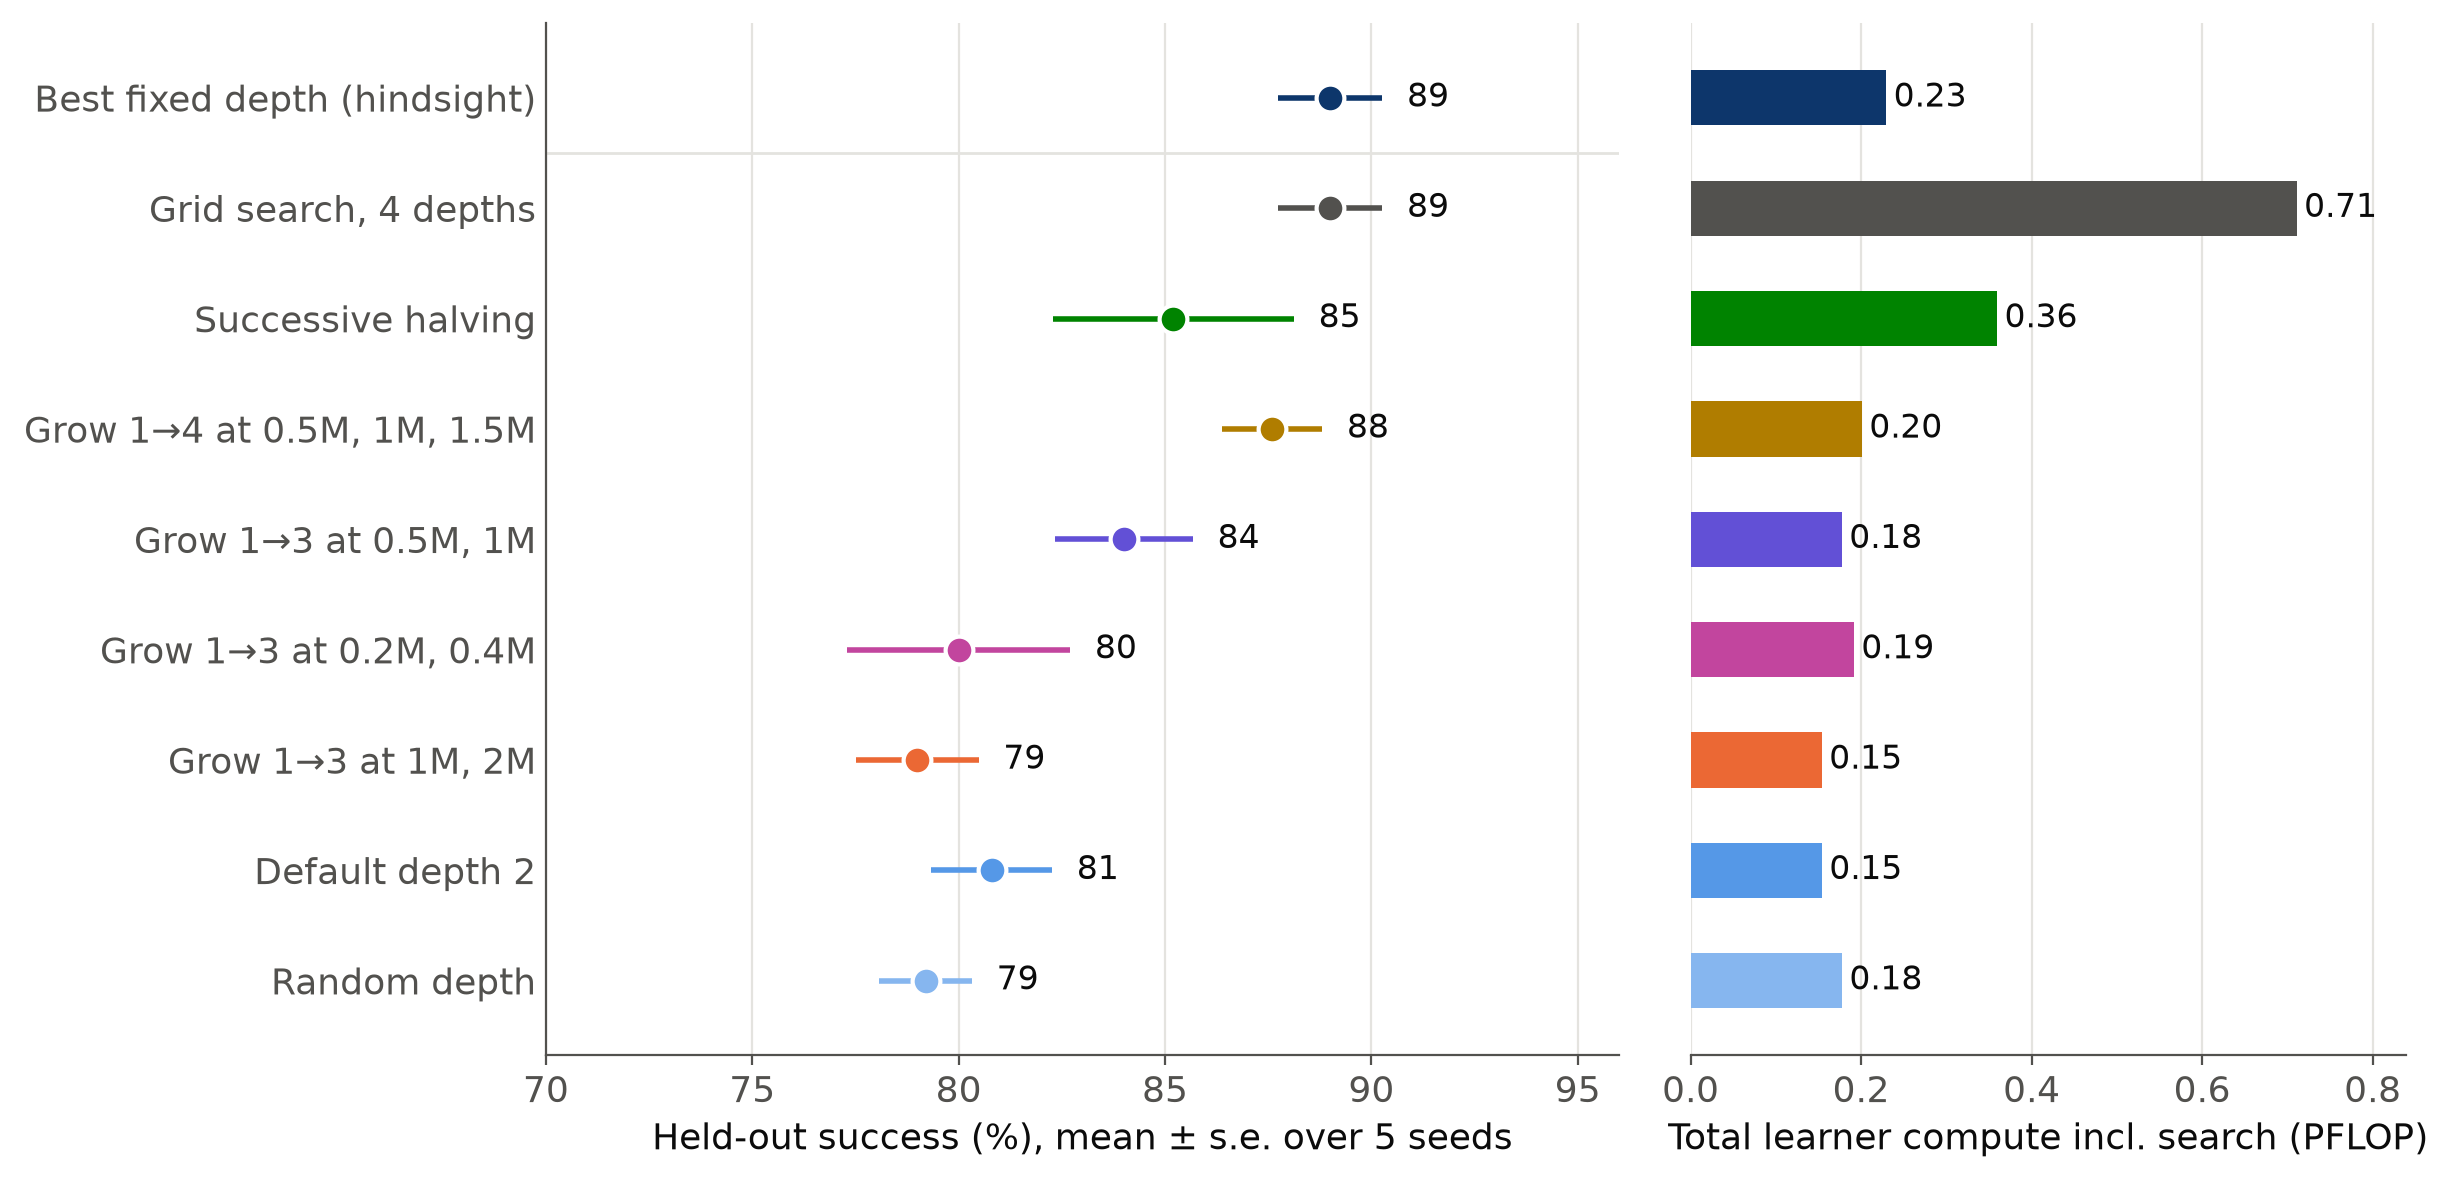
\includegraphics[width=0.85\linewidth]{w400/strategy_panel.png}
    \caption{Held-out success (left, mean $\pm$ s.e.\ over five paired seeds) and total learner compute including all runs a strategy trains (right), width 400.}
    \label{fig:strategy}
\end{figure}

\begin{figure}[!t]
    \centering
    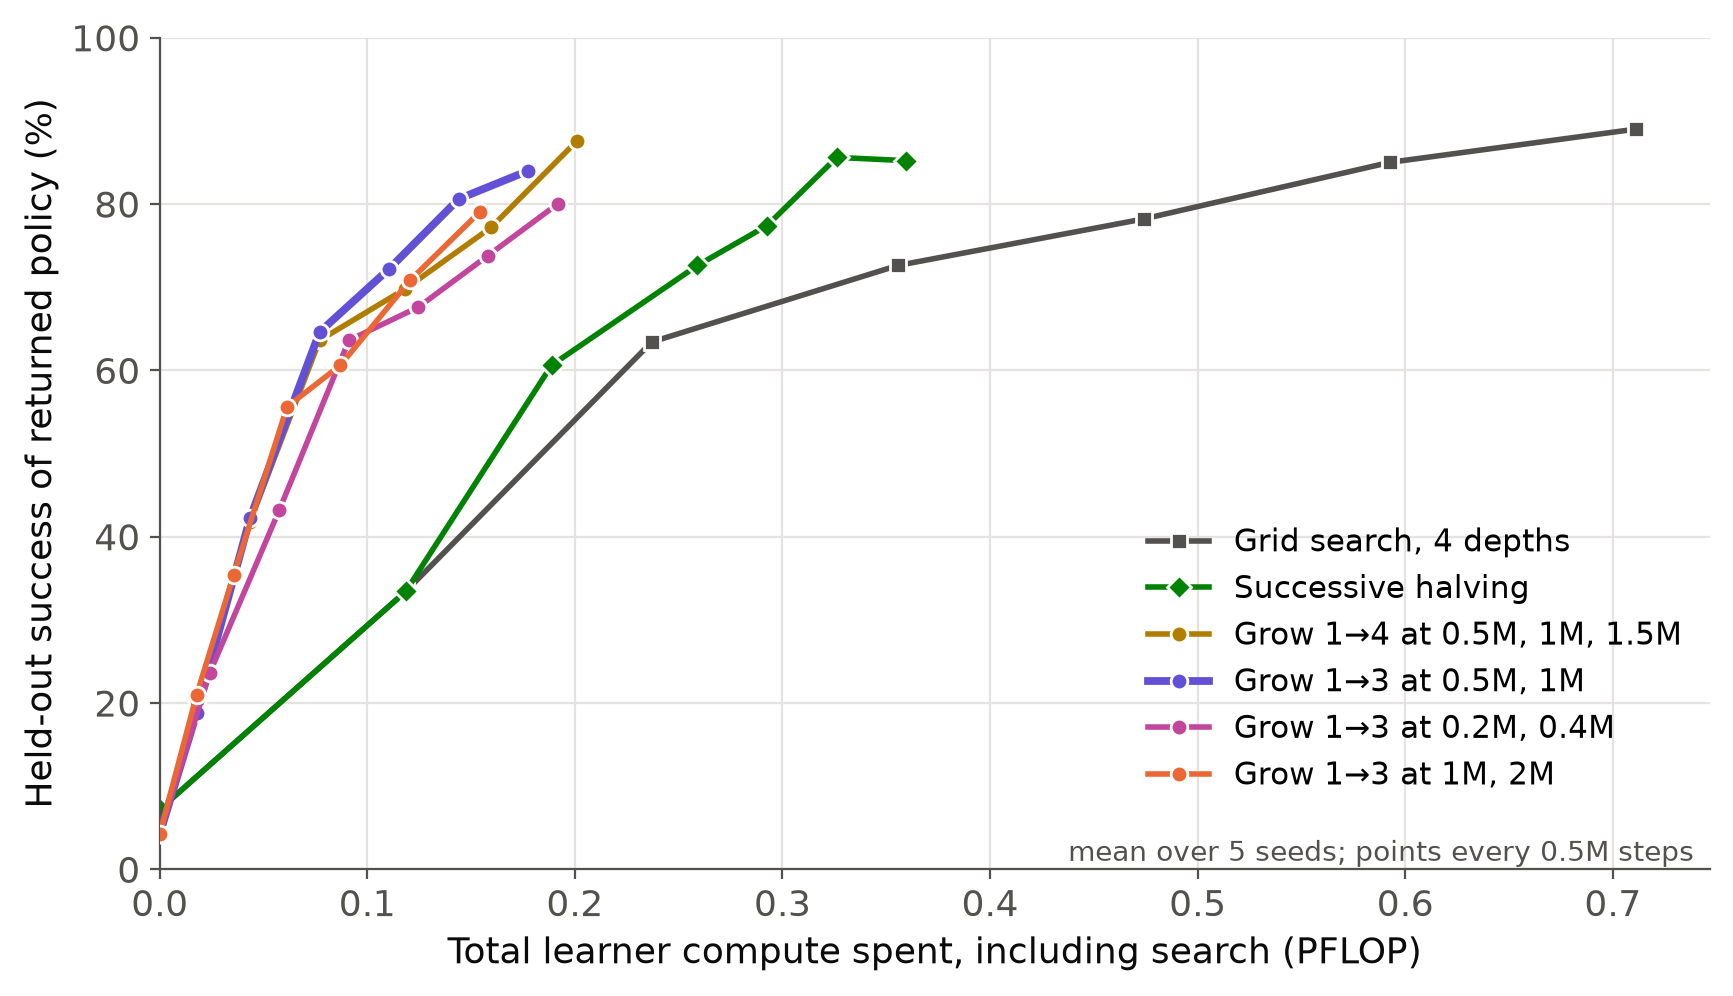
\includegraphics[width=0.58\linewidth]{w400/anytime_flops.png}
    \caption{Held-out success of the policy each strategy would return if stopped at a given total compute, mean over five seeds, width 400. Search strategies pay for all their candidate runs in parallel; a growing run pays for one network that is small at first.}
    \label{fig:anytime}
\end{figure}

\paragraph{Growth versus search.}
Table~\ref{tab:main} and Figure~\ref{fig:strategy} compare the strategies.
\growF{} reaches $87.6\%$ in one run, $1.4 \pm 4.4$ points below grid search and the best fixed depth, and $2.4 \pm 10.0$ points above successive halving; neither difference is resolved with five seeds.
It costs 0.20 PFLOP: 28\% of grid search (0.71), 56\% of successive halving (0.36) and less than a single fixed depth-4 run (0.25), because it trains a depth-1 network for its first 0.5M steps.
It is better than committing to the default depth ($+6.8 \pm 5.2$) or to a random depth ($+8.4 \pm 5.1$).
\growE{}, which stops at depth 3, reaches 84.0\%, comparable to successive halving at half its compute but $5.0 \pm 3.7$ points below the best depth; most of that gap closes when growth continues to the largest candidate depth ($+3.6 \pm 5.9$ for \growF{} over \growE{}, not resolved).
Per task, \growF{} solves \texttt{peg-insert-side} in all seeds (100\%, against 76\% for fixed depth 4) but reaches 64\% on \texttt{push}, where depth 4 reaches 88\% (Figure~\ref{fig:pertask}).
Figure~\ref{fig:anytime} shows the same comparison over the course of training: at every compute level up to 0.2 PFLOP, the growing runs return a better policy than either search, which at that point is still paying for four candidate networks.
Successive halving does not reach the final success of \growF{} within its budget (at most 85.6\%), and grid search exceeds it only at the end of its budget (0.71 PFLOP, 3.5 times as much).

\begin{table}[!t]
    \caption{Width 128, five paired seeds; same protocol as Table~\ref{tab:main}. Here depth 3 is the best fixed depth on average.}
    \label{tab:w128}
    \centering
    \small
    \begin{tabular}{lccc}
        \toprule
        Strategy & Success (\%) & Env.\ steps (M) & Learner PFLOP \\
        \midrule
        Grid search, depths 1--4          & $81.0 \pm 1.1$ & 12.0 & 0.44 \\
        Successive halving (simulated)    & $77.8 \pm 2.1$ & 5.5  & 0.21 \\
        Default depth 2                   & $72.2 \pm 2.6$ & 3.0  & 0.11 \\
        Random depth (mean of 1--4)       & $71.2 \pm 0.8$ & 3.0  & 0.11 \\
        \midrule
        \growF{} (1$\to$4 at 0.5M, 1M, 1.5M) & $76.2 \pm 2.7$ & 3.0 & 0.11 \\
        \growE{} (1$\to$3 at 0.5M, 1M)    & $73.6 \pm 1.7$ & 3.0  & 0.11 \\
        \growL{} (1$\to$3 at 1M, 2M)      & $69.6 \pm 2.9$ & 3.0  & 0.11 \\
        \midrule
        Best fixed depth$^\dagger$        & $81.0 \pm 1.1$ & 3.0  & 0.11 \\
        \bottomrule
    \end{tabular}
\end{table}

\paragraph{A narrower actor: width 128.}
To check the rule ``grow to the largest candidate depth'' where the largest depth is not the best, we repeated the fixed depths and three schedules with width-128 actors (Table~\ref{tab:w128}).
Fixed depths reach 59.0\%, 72.2\%, 79.2\% and 74.6\% at depths 1--4; the best depth in hindsight is 3 for three seeds and 2 and 4 for one each, and validation again selects it in all five seeds.
All 35 identity insertions left the action mean unchanged.
\growF{} reaches 76.2\%, $4.8 \pm 8.0$ points below grid search and $1.6 \pm 9.7$ below successive halving, at 26\% and 55\% of their compute.
Its advantage over the default depth ($+4.0 \pm 6.6$) and a random depth ($+5.0 \pm 7.3$) is smaller than at width 400 and not resolved.
The ordering of the schedules is the same as at width 400: \growF{} is above \growE{} ($+2.6 \pm 5.8$), which is above \growL{} ($+4.0 \pm 7.5$), although none of these differences is resolved.
At this width, growth therefore remained a cheap option but did not clearly match search (Figure~\ref{fig:w128} in the appendix).

\FloatBarrier
\section{Discussion and limitations}

\paragraph{What the results support.}
When the right depth is unknown, growing early to the largest candidate depth was, at width 400, as good as searching over depths at a fraction of the compute; at width 128 it was cheaper but on average 4.8 points worse.
Two design choices were necessary: identity initialisation, which avoids a collapse of the policy at insertion, and early insertion, which leaves enough of the budget to train the deeper network.
The second observation is consistent with work showing that capacity added late in RL training is harder to use \citep{nikishin2022primacy,lyle2023plasticity}, although we did not measure plasticity directly.

\paragraph{Limitations.}
This is a small study.
It uses one benchmark, one algorithm, a 3M-step budget and five seeds per configuration, and per-run success estimates from 100 held-out episodes carry roughly $\pm 4$ points of binomial noise; several differences we report are within seed-to-seed variation and are marked as unresolved.
The \growF{} schedule was added after we saw that depth 4 was the best fixed depth at width 400; the rule it follows, growing to the largest candidate depth, does not use test results, but it was not chosen blind.
At width 128 the same schedule stayed 4.8 points below grid search on average, so we cannot claim that growth matches search in general, only that it did so at width 400 within the resolution of five seeds.
Growth follows fixed schedules rather than an adaptive trigger, and only the actor grows.
Successive halving is simulated from logged curves with one rung schedule.
Held-out goals test interpolation within tasks, not generalisation to new tasks.

\paragraph{Next steps.}
The most direct extensions are growth triggered by a plateau in validation success, growing the critic, larger depth ranges, and MT50, where interference between tasks may make capacity more important.

\section{Conclusion}

Function-preserving identity insertion lets a multi-task PPO policy grow deeper with no change at insertion, while random initialisation of the same layers causes a large drop that the run never fully recovers from.
On Meta-World MT10 with width-400 actors, where depth is worth 24 points of held-out success, growing early to the largest candidate depth reached the performance of the best fixed depth to within the resolution of five seeds, at 28\% of the compute of grid search and 56\% of successive halving.
At width 128 the same schedule was 4.8 points below grid search on average, so the result does not carry over unchanged. Counting the cost of the search, growth is a cheap alternative to choosing depth by search, provided that layers are added as the identity and early in training.

\bibliographystyle{plainnat}
\bibliography{refs}

\clearpage
\appendix

\section{Additional results}

\begin{figure}[!htbp]
    \centering
    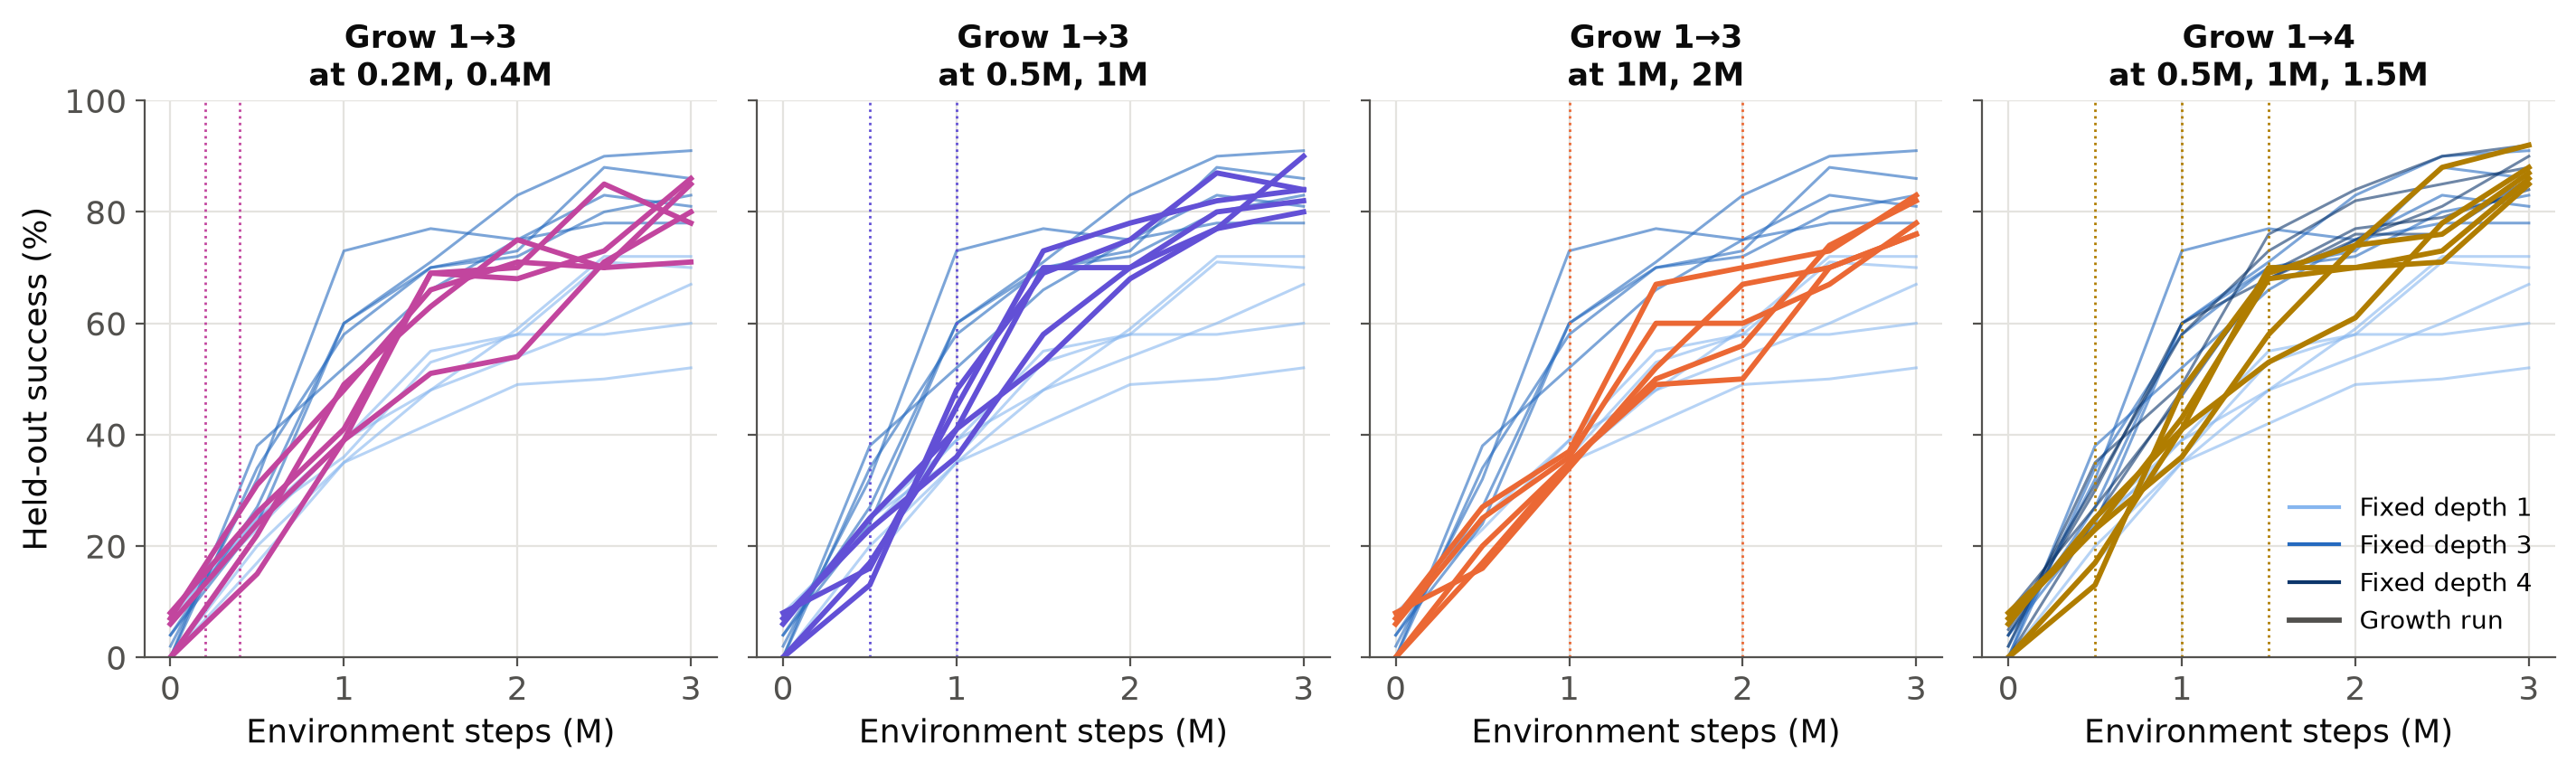
\includegraphics[width=\linewidth]{w400/growth_traj.png}
    \caption{Held-out success of every growth run (bold, one line per seed) against the fixed-depth runs of all seeds (thin). Dotted lines mark insertions. Width 400.}
    \label{fig:traj}
\end{figure}

\begin{figure}[!htbp]
    \centering
    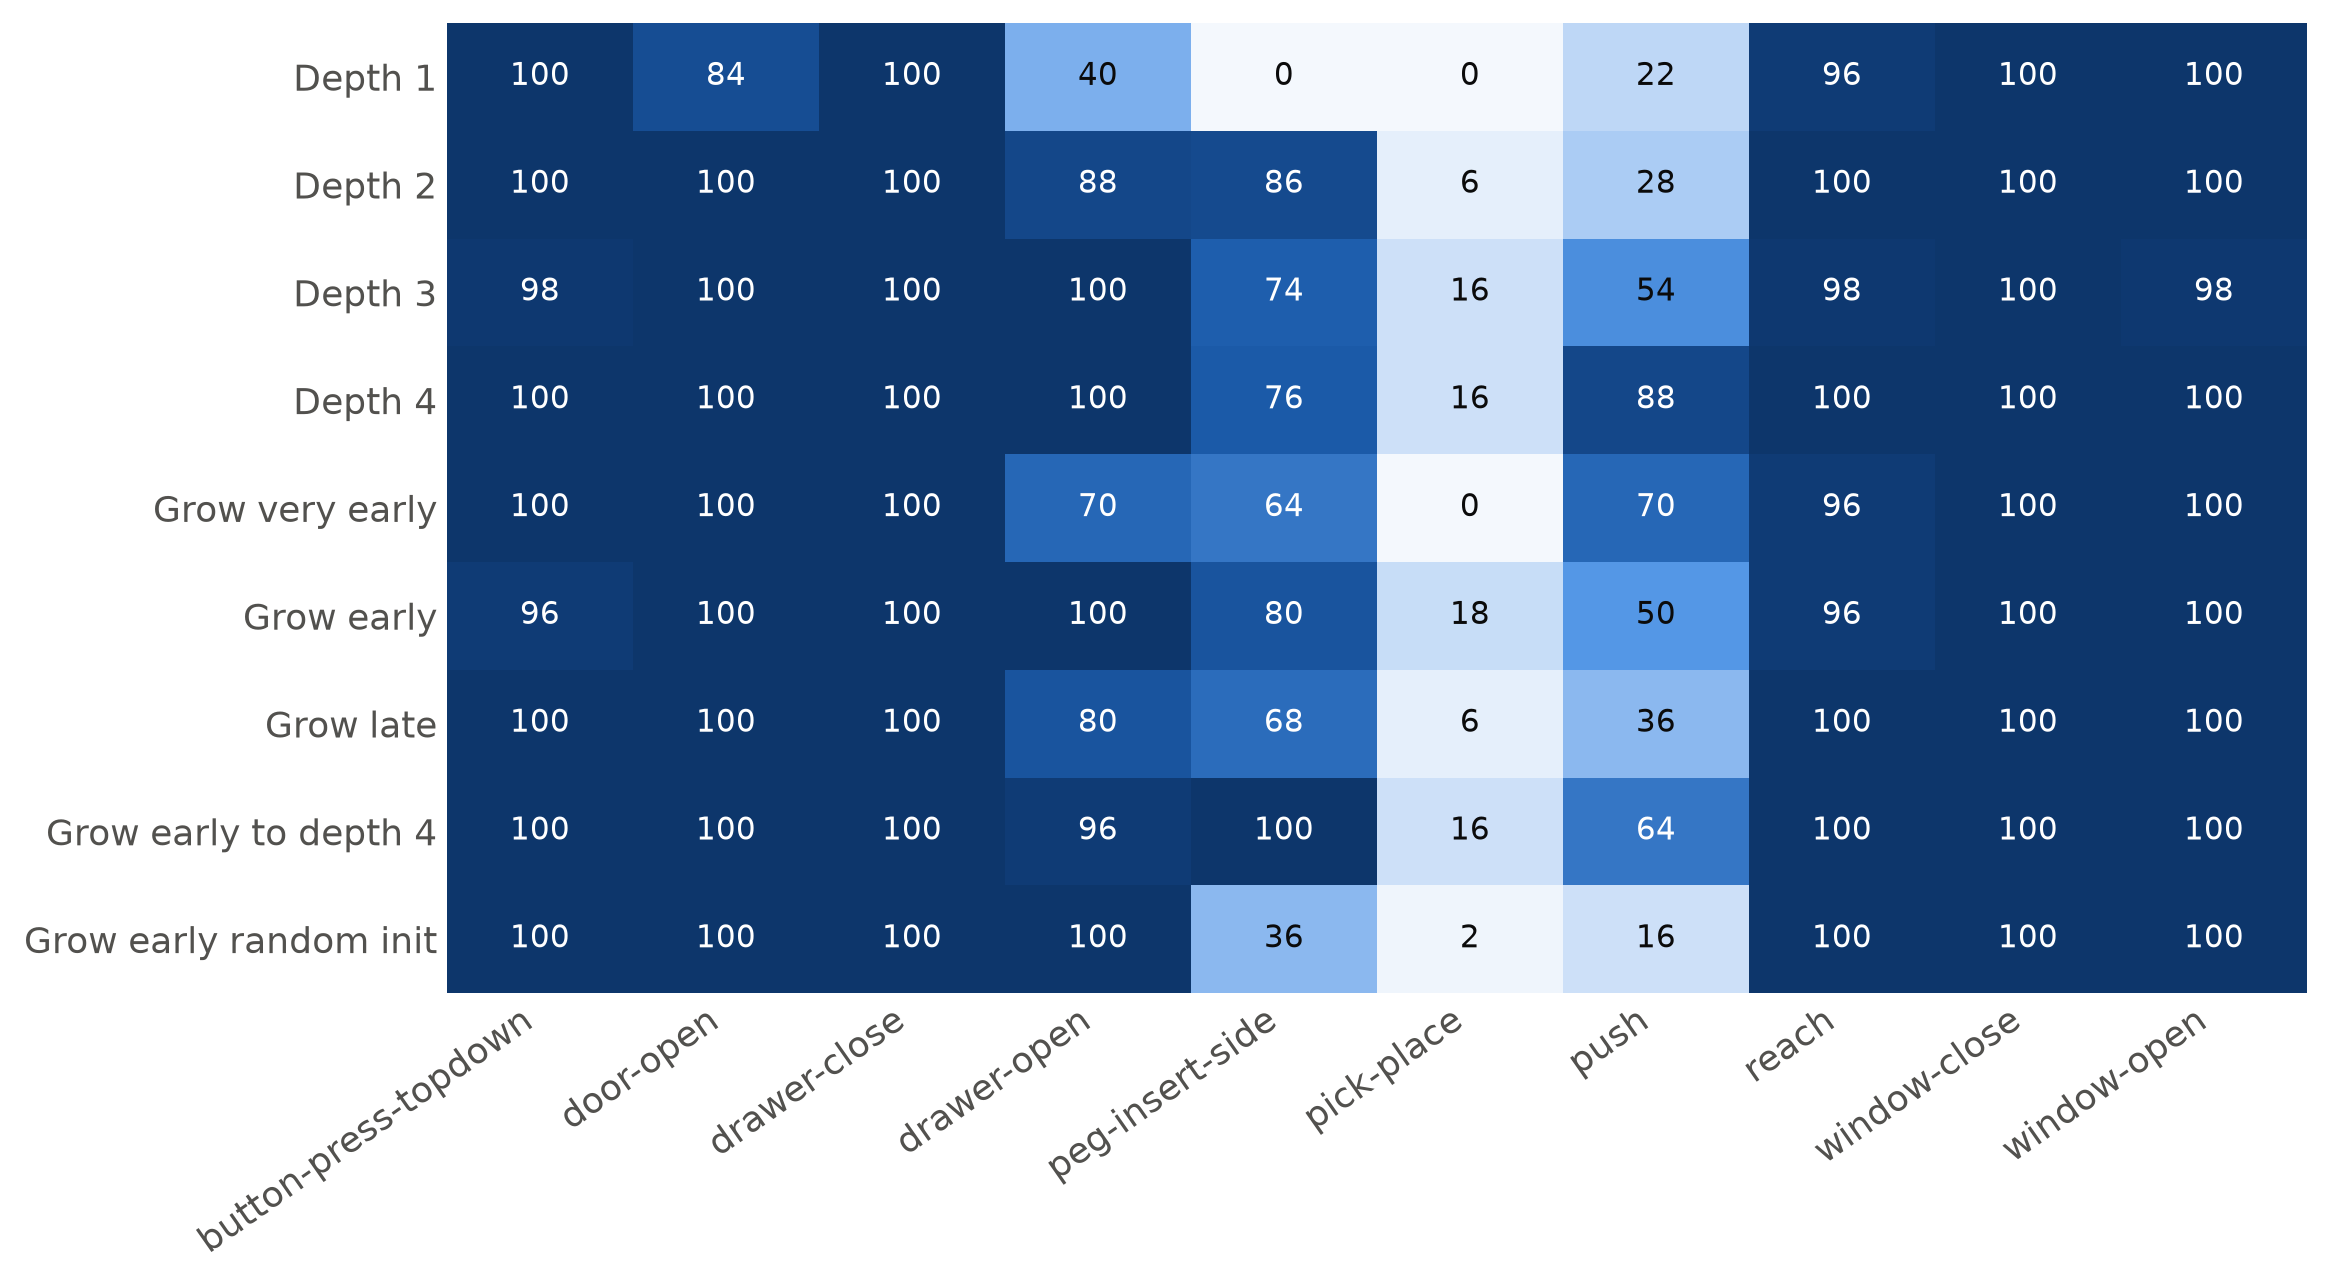
\includegraphics[width=\linewidth]{w400/per_task.png}
    \caption{Final held-out success per task (\%), mean over five seeds, width 400.}
    \label{fig:pertask}
\end{figure}

\begin{table}[!htbp]
    \caption{Final held-out success (\%) of every width-400 run, by seed.}
    \label{tab:seeds}
    \centering
    \resizebox{\linewidth}{!}{%
    \begin{tabular}{lccccccccc}
        \toprule
        Seed & D1 & D2 & D3 & D4 & \growVE{} & \growE{} & \growL{} & \growF{} & \growR{} \\
        \midrule
        1 & 60 & 86 & 91 & 88 & 78 & 82 & 78 & 86 & 71 \\
        2 & 72 & 79 & 81 & 92 & 71 & 90 & 83 & 87 & 79 \\
        3 & 67 & 82 & 78 & 90 & 85 & 84 & 82 & 92 & 72 \\
        4 & 70 & 79 & 83 & 86 & 86 & 84 & 76 & 85 & 81 \\
        5 & 52 & 78 & 86 & 84 & 80 & 80 & 76 & 88 & 74 \\
        \midrule
        Mean & 64.2 & 80.8 & 83.8 & 88.0 & 80.0 & 84.0 & 79.0 & 87.6 & 75.4 \\
        \bottomrule
    \end{tabular}}
\end{table}

\begin{table}[!htbp]
    \caption{Final held-out success (\%) of every width-128 run, by seed.}
    \label{tab:seeds128}
    \centering
    \small
    \begin{tabular}{lccccccc}
        \toprule
        Seed & D1 & D2 & D3 & D4 & \growE{} & \growL{} & \growF{} \\
        \midrule
        1 & 56 & 73 & 76 & 81 & 70 & 60 & 70 \\
        2 & 57 & 76 & 84 & 73 & 72 & 72 & 82 \\
        3 & 68 & 63 & 83 & 79 & 76 & 78 & 74 \\
        4 & 55 & 71 & 79 & 69 & 71 & 70 & 72 \\
        5 & 59 & 78 & 74 & 71 & 79 & 68 & 83 \\
        \midrule
        Mean & 59.0 & 72.2 & 79.2 & 74.6 & 73.6 & 69.6 & 76.2 \\
        \bottomrule
    \end{tabular}
\end{table}

\begin{figure}[!htbp]
    \centering
    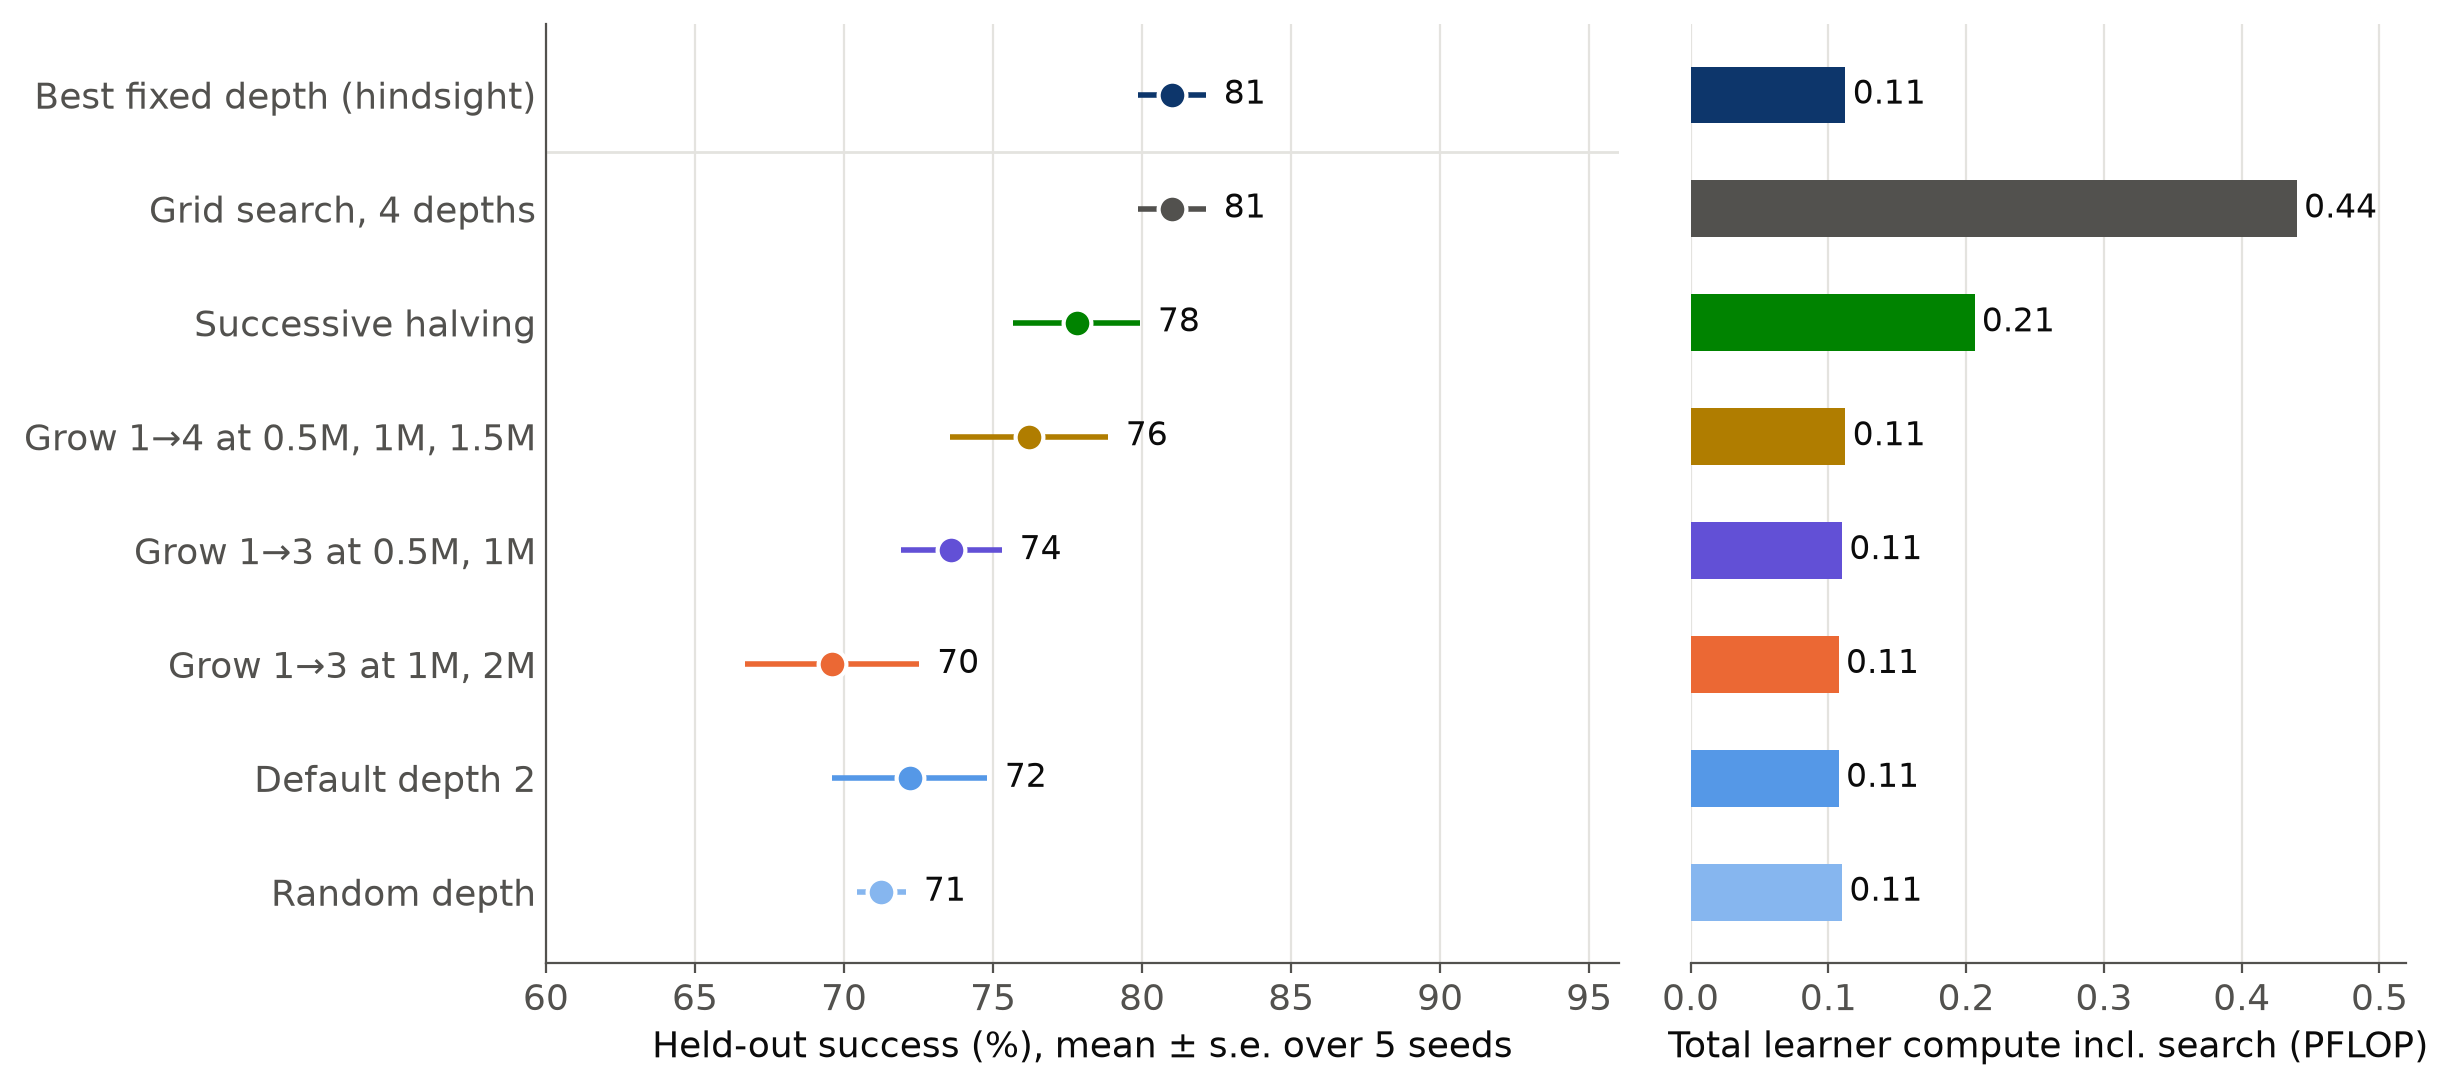
\includegraphics[width=\linewidth]{w128/strategy_panel.png}
    \caption{Held-out success and total learner compute of each strategy, width 128, five paired seeds.}
    \label{fig:w128}
\end{figure}

\begin{figure}[!htbp]
    \centering
    \begin{subfigure}[t]{0.49\linewidth}
        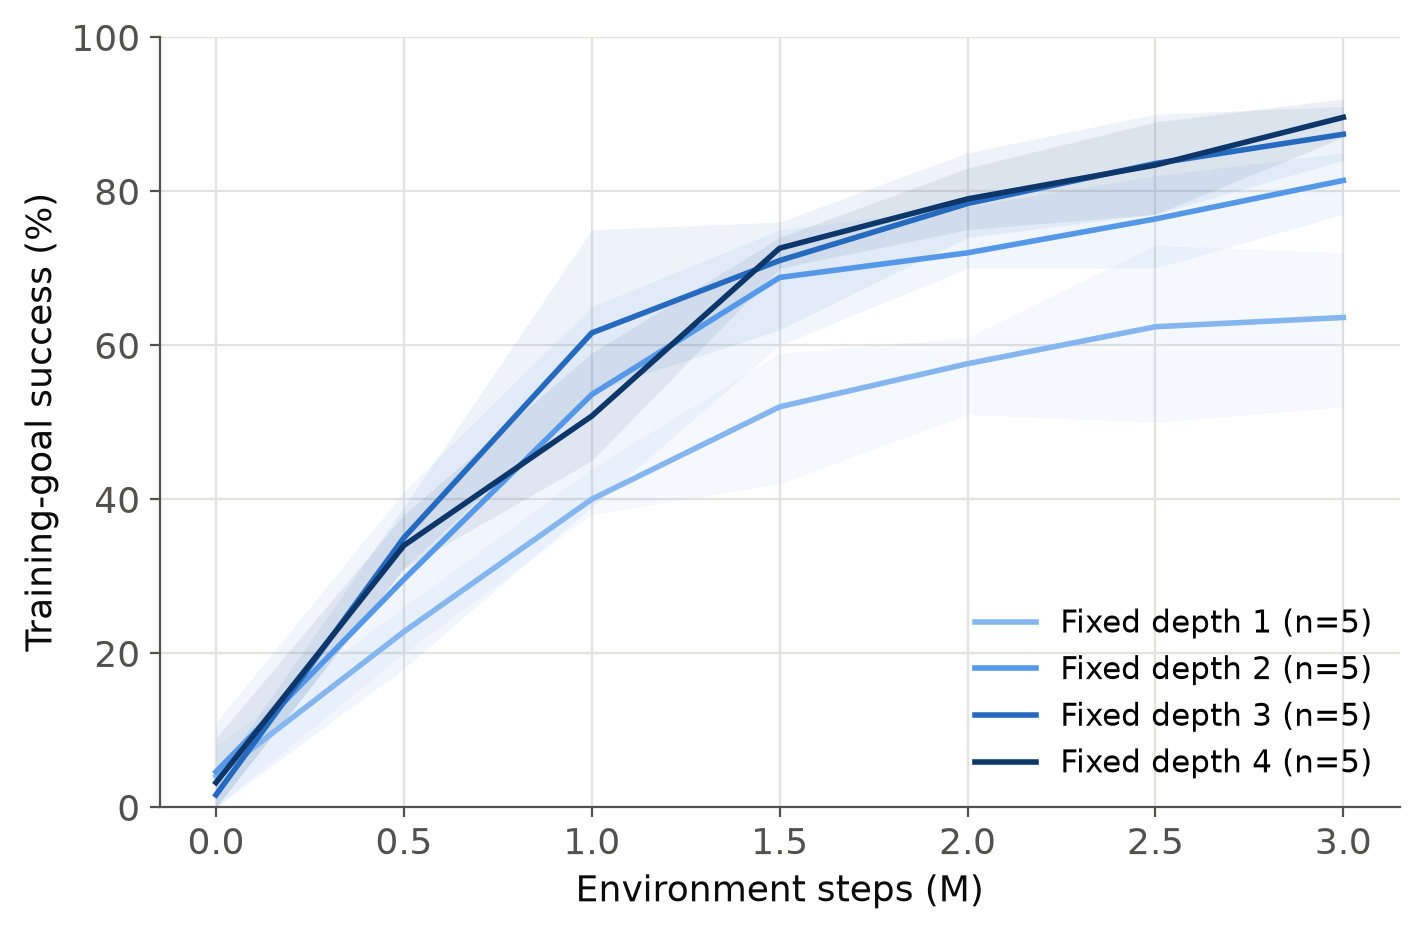
\includegraphics[width=\linewidth]{w400/curves_success_train.png}
        \caption{Training goals}
    \end{subfigure}\hfill
    \begin{subfigure}[t]{0.49\linewidth}
        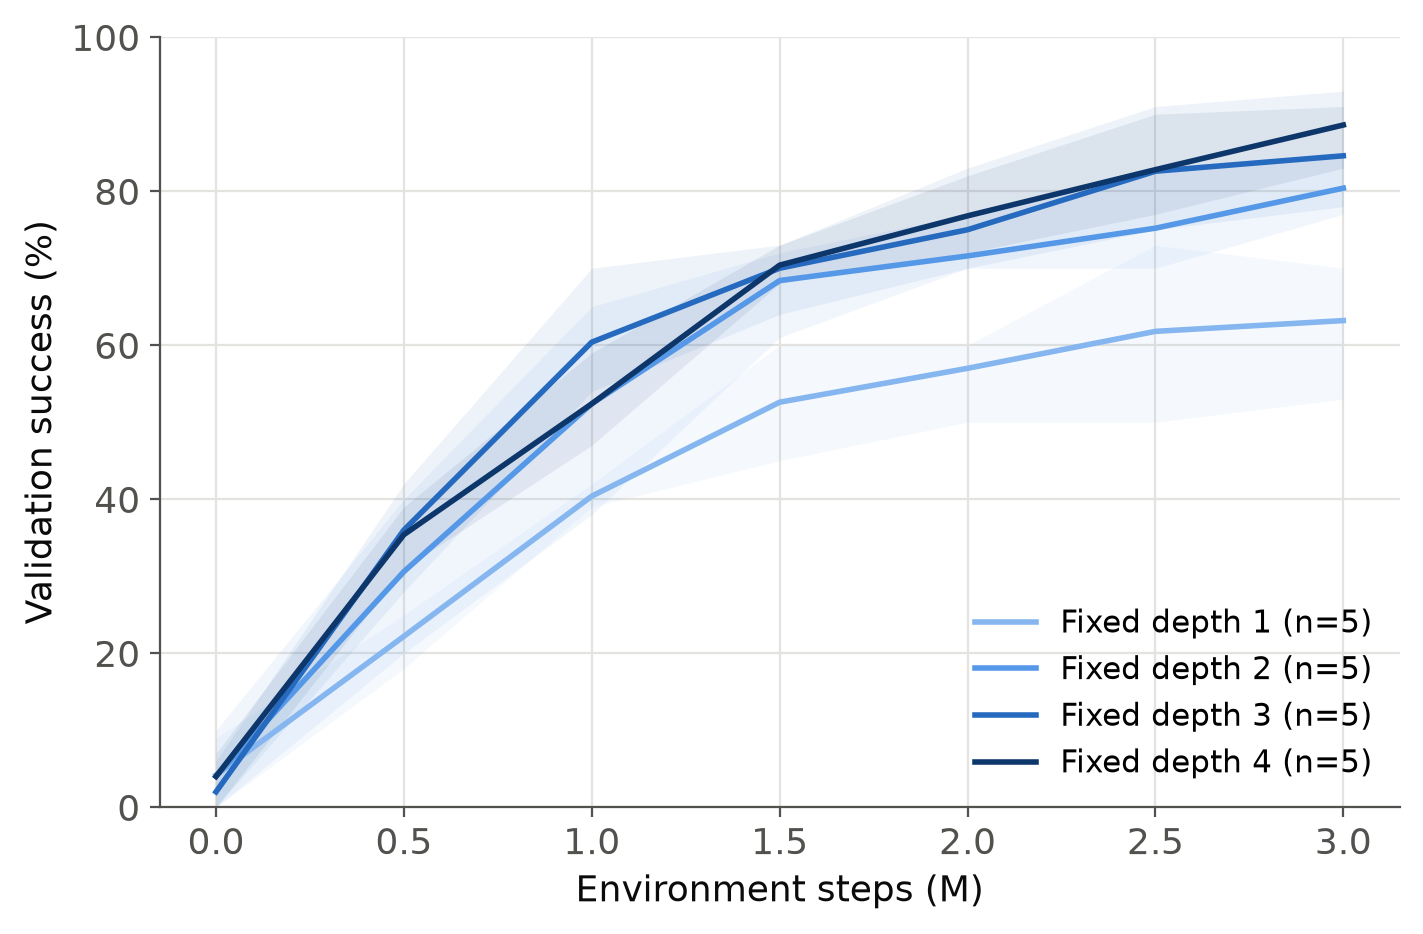
\includegraphics[width=\linewidth]{w400/curves_success_dev.png}
        \caption{Validation goals}
    \end{subfigure}
    \caption{Learning curves of the fixed depths on training and validation goals, width 400.}
\end{figure}

\begin{figure}[!htbp]
    \centering
    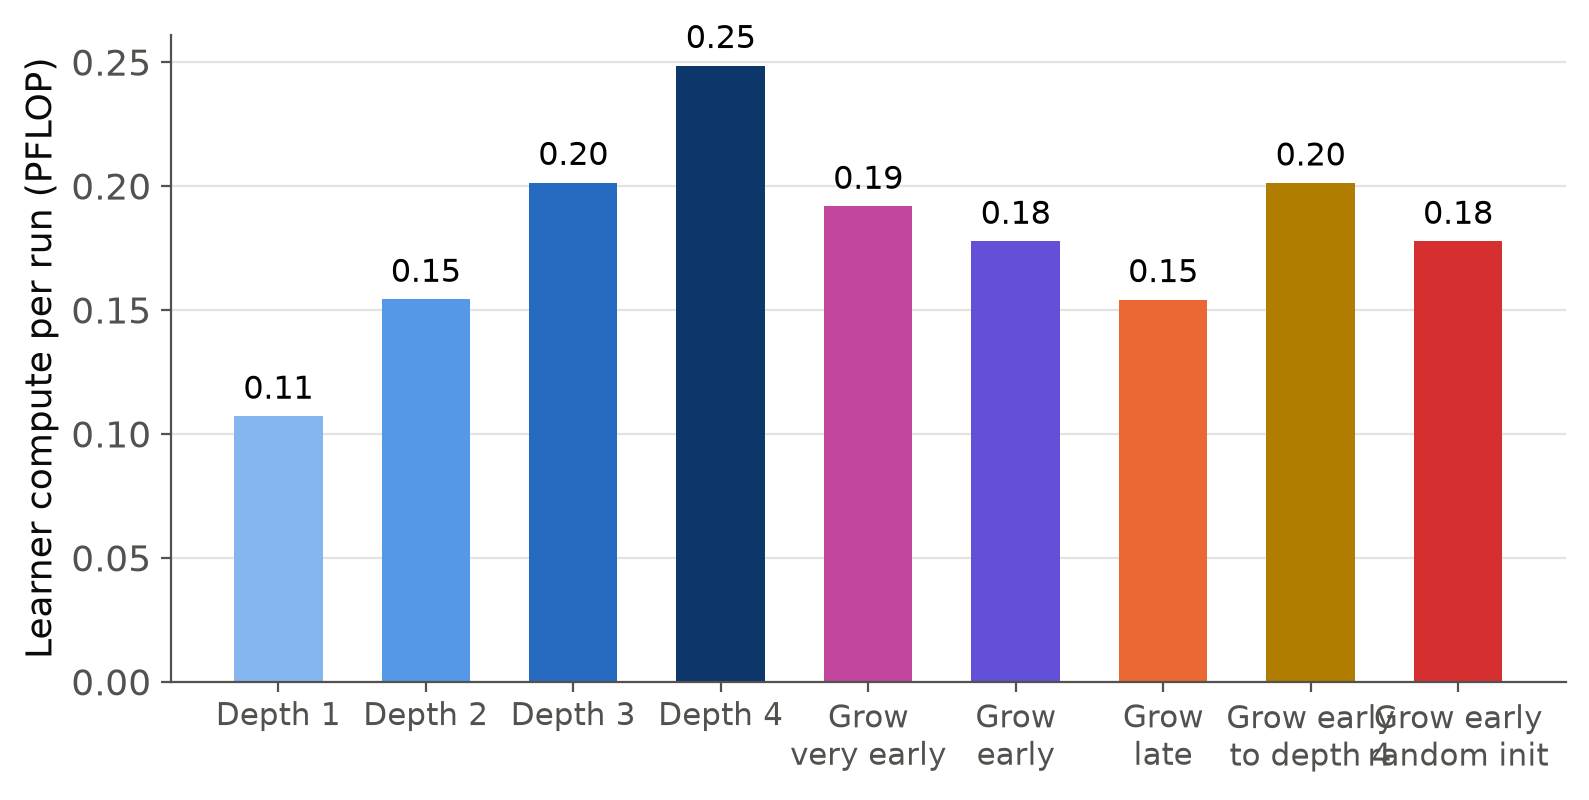
\includegraphics[width=0.85\linewidth]{w400/flops_per_run.png}
    \caption{Learner compute of a single 3M-step run of each configuration, width 400.}
    \label{fig:flops}
\end{figure}

\paragraph{Reproducibility.}
The repository (\coderepo) contains the runner (\texttt{runner/}), a script that lists every reported run (\texttt{scripts/run\_study.sh}), the logs of all 80 runs (\texttt{results/runs/}: configuration, final state, evaluations every 0.5M steps, per-rollout metrics and insertion events), and the scripts that produce every figure and number in this report from those logs.
Dependency versions are pinned in \texttt{runner/resolved.lock} (Python 3.12, PyTorch 2.8, Meta-World 3.0, MuJoCo 3.7, Tianshou 2.0).
One configuration (width 400, depth 4, seed 2) was trained twice after a cloud job appeared to fail and later completed (92\% and 91\%); we report the first.

\end{document}
